\begin{savequote}[45mm]
\ascii{Any fool can write code that a computer can understand. Good programmers write code that humans can understand.}
\qauthor{\ascii{- Martin Flower}}
\end{savequote}

\chapter{本地执行} 
\label{ch:local}

\begin{content}

\tf{}可以独立地运行在一个进程内,完成计算图的执行过程。本章将重点介绍本地运行时的基本架构与运行机制;重点讨论计算图剪枝、分裂、优化、执行等实现技术细节;并且详细探究在本地模式下,跨设备间\ascii{OP}之间数据交互的工作机制,及其\ascii{OP}在设备集上的编排(\ascii{placement})算法。

\end{content}

\section{本地模式}
\label{sec:local-runtime}

\begin{content}

如\refig{local}所示,在本地模式下,\ascii{Client, Master, Worker}部署在同一台机器同一进程内,并由\code{DirectSession}同时扮演这三个角色。\code{DirectSession}运行在单独的进程内,各服务实体之间是函数调用关系。

\begin{figure}[H]
\centering
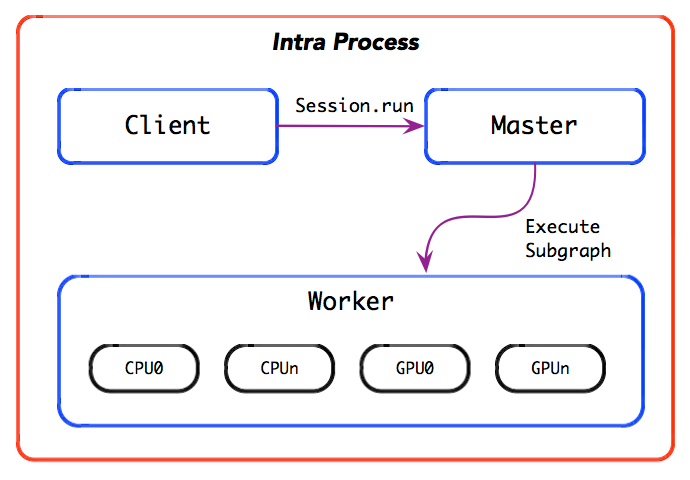
\includegraphics[width=0.7\textwidth]{figures/local.png}
\caption{本地模式}
 \label{fig:local}
\end{figure}

\ascii{Client}负责计算图的构造,通过调用\code{Session.run},启动计算图的执行过程。如\refig{local-runtime}所示,在\code{run\_step}执行过程之中,涉及计算图的剪枝、分裂、执行三个重要阶段。

\begin{figure}[H]
\centering
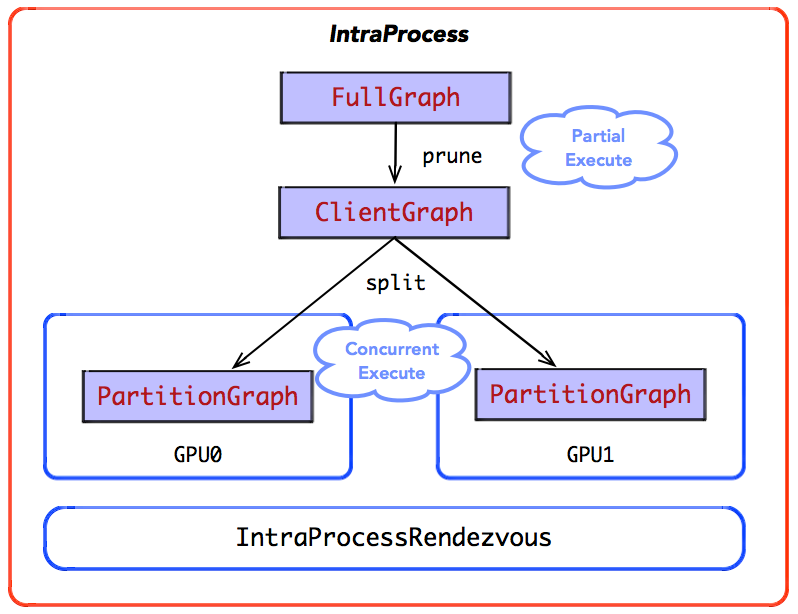
\includegraphics[width=0.8\textwidth]{figures/local-runtime.png}
\caption{本地模式:图操作}
 \label{fig:local-runtime}
\end{figure}

\subsection{部分执行}

\ascii{Master}收到计算图执行命令后,启动计算图的剪枝操作。它根据计算图的输入输出反向遍历图,寻找一个最小依赖的子图,常称为\code{ClientGraph}。

也就是说,每次执行\code{run\_step}时,并不会执行整个计算图(\code{FullGraph}),而是执行部分的子图。剪枝体现了\tf{}部分执行的设计理念。

\subsection{并发执行}

然后,运行时按照当前设备集完成图的分裂,生成了很多子图,每个子图称为\code{PartitionGraph};然后触发各个\ascii{Worker}并发地执行每个\code{PartitionGraph};对于每一个\ascii{PartitionGraph},运行时将启动一个\ascii{Executor},按照其拓扑排序完成\code{PartitionGraph}的执行。

也就是说,分裂和执行体现了\tf{}并发执行的设计理念。

\section{会话控制}

在本地模式下,其运行时由\code{DirectSession}控制。一般地,\code{DirectSession}执行计算图时,各组件之间都是函数调用关系。但是,\code{DirectSession}也存在清晰的生命周期管理机制,如\refig{local-direct-session-lifecycle}所示。

\begin{figure}[H]
\centering
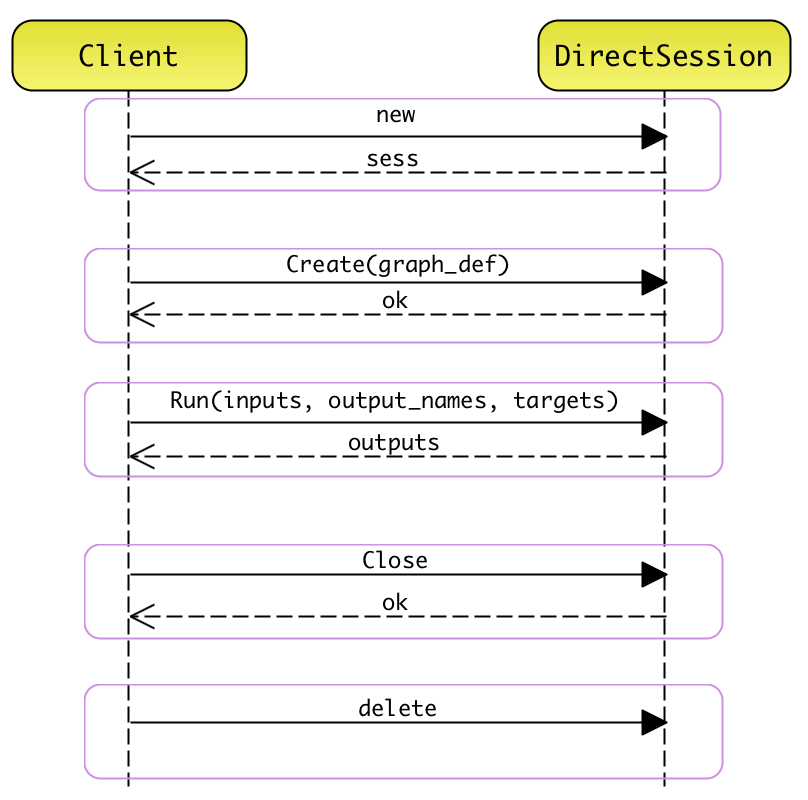
\includegraphics[width=0.6\textwidth]{figures/local-direct-session-lifecycle.png}
\caption{DirectSession生命周期}
 \label{fig:local-direct-session-lifecycle}
\end{figure}

\subsection{领域模型}

如\refig{local-direct-session-model}所示,\code{DirectSession}持有\code{SimpleGraphExecutionState}实例,后者负责计算图的剪枝,生成\code{ClientGraph}实例。

\code{DirectSession}同时持有一组线程池,但是没次\code{DirectSession.run}时,根据外部配置的索引,从线程池组里选择其一为其提供服务。因为\code{DirectSession}是线程安全的,支持多个并发执行的\code{DirectSession.run},即可以同时运行多个线程池实例。

\begin{figure}[H]
\centering
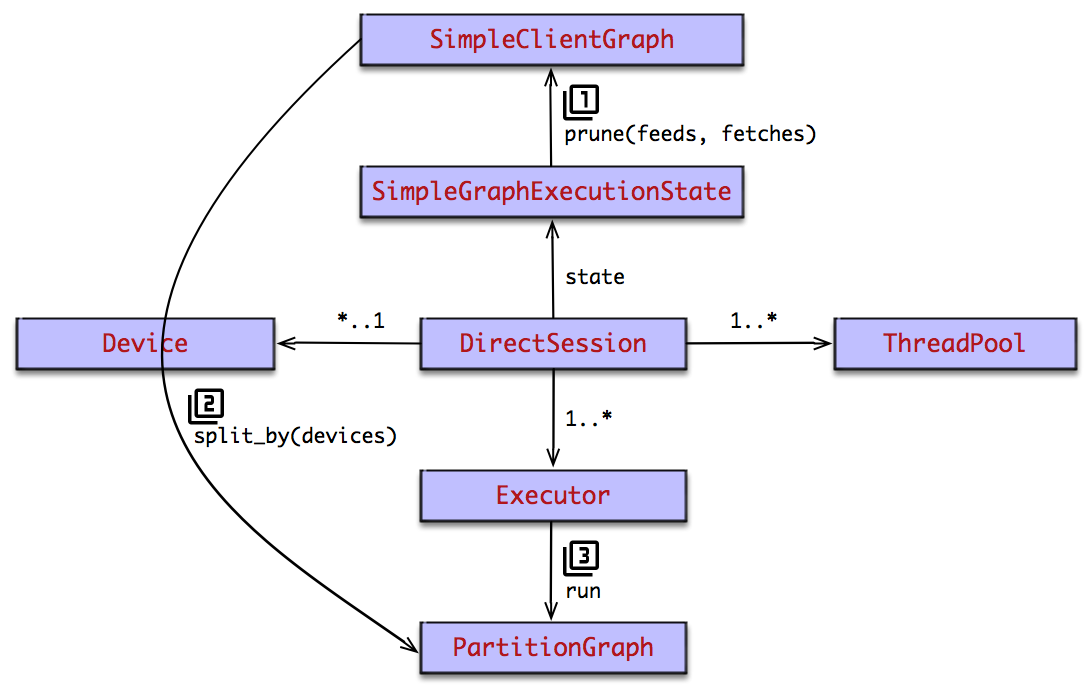
\includegraphics[width=0.9\textwidth]{figures/local-direct-session-model.png}
\caption{DirectSession领域模型}
 \label{fig:local-direct-session-model}
\end{figure}

\subsection{创建会话}

如\refig{local-direct-session-factory}所示,\code{DirectSession}由\code{DirectSessionFactory}多态创建。其中,\code{DeviceFactory::AddDevices}将创建本地设备集。

其中,\code{DirectSession}中主要完成线程池组的创建。

\begin{figure}[H]
\centering
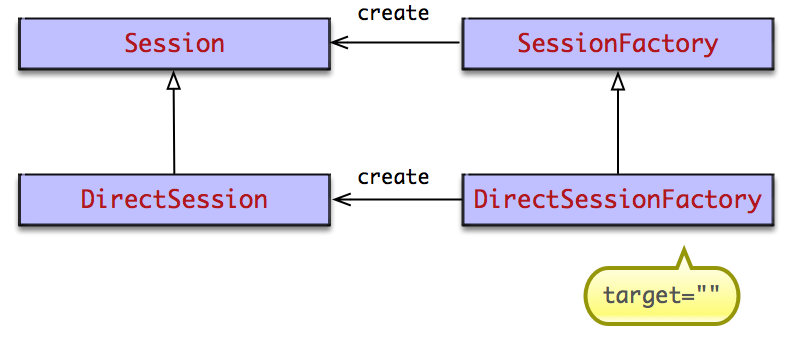
\includegraphics[width=0.6\textwidth]{figures/local-direct-session-factory.png}
\caption{多态创建DirectSession}
 \label{fig:local-direct-session-factory}
\end{figure}

\begin{leftbar}
\begin{c++}
struct DirectSessionFactory : SessionFactory {
  bool AcceptsOptions(const SessionOptions& options) override {
    return options.target.empty();
  }

  Session* NewSession(const SessionOptions& options) override {
    std::vector<Device*> devices;
    DeviceFactory::AddDevices(
        options, "/job:localhost/replica:0/task:0", &devices);
    return new DirectSession(options, new DeviceMgr(devices));
  }
};
\end{c++}
\end{leftbar}

其中,\code{DirectSessionFactory::NewSession}由\ascii{C API}调用。

\begin{leftbar}
\begin{c++}
Status NewSession(const SessionOptions& options, Session** out_session) {
  SessionFactory* factory;
  Status s = SessionFactory::GetFactory(options, &factory);
  if (!s.ok()) {
    *out_session = nullptr;
    return s;
  }
  *out_session = factory->NewSession(options);
  if (!*out_session) {
    return errors::Internal("Failed to create session.");
  }
  return Status::OK();
}

TF_DeprecatedSession* TF_NewDeprecatedSession(
  const TF_SessionOptions* opt, TF_Status* status) {
  Session* session;
  status->status = NewSession(opt->options, &session);
  if (status->status.ok()) {
    return new TF_DeprecatedSession({session});
  } else {
    return nullptr;
  }
}
\end{c++}
\end{leftbar}

在\code{DirectSession}的构造函数中,主要负责其领域模型的初始化,包括线程池的创建,构建\code{CancellationManager}实例。

\begin{leftbar}
\begin{c++}
DirectSession::DirectSession(
    const SessionOptions& options,
    const DeviceMgr* device_mgr)
    : options_(options),
      device_mgr_(device_mgr),
      cancellation_manager_(new CancellationManager()) {
  // thread\_pools\_ = ... 
}
\end{c++}
\end{leftbar}

\subsection{销毁会话}

由\ascii{SessionFactory}所\code{new}出来的\code{DirectSession},由\ascii{C API}负责\code{delete}掉。

\begin{leftbar}
\begin{c++}
void TF_DeleteDeprecatedSession(TF_DeprecatedSession* s, TF_Status* status) {
  status->status = Status::OK();
  delete s->session;  // delete DirectSession
  delete s;
}
\end{c++}
\end{leftbar}

随后,\code{DirectSession}的析构函数被调用,它负责清理其负责管理的系统资源。主要包括\code{Executor}列表,\code{ThreadPool}列表,\code{CancellationManager}实例。

\begin{leftbar}
\begin{c++}
DirectSession::~DirectSession() {
  for (auto& it : partial_runs_) {
    it.second.reset(nullptr);
  }
  
  for (auto& it : executors_) {
    it.second.reset();
  }
  
  for (auto d : device_mgr_->ListDevices()) {
    d->op_segment()->RemoveHold(session_handle_);
  }
  
  delete cancellation_manager_;
  
  for (const auto& p_and_owned : thread_pools_) {
    if (p_and_owned.second) delete p_and_owned.first;
  }

  execution_state_.reset(nullptr);
  flib_def_.reset(nullptr);
}
\end{c++}
\end{leftbar}

\subsection{创建/扩展图}

首次扩展图,等价于创建图。扩展图就是在原有计算图的基础上,追加新的子图。当然,追加的子图中所包含的节点,在原有的计算图中不应该存在。


\begin{leftbar}
\begin{c++}
Status DirectSession::Create(const GraphDef& graph) {
  if (graph.node_size() > 0) {
    mutex_lock l(graph_def_lock_);
    return ExtendLocked(graph);
  }
  return Status::OK();
}

Status DirectSession::Extend(const GraphDef& graph) {
  mutex_lock l(graph_def_lock_);
  return ExtendLocked(graph);
}
\end{c++}
\end{leftbar}

当创建计算图时,\code{DirectSession}主要完成\code{SimpleGraphExecutionState}实例的创建。如\refig{local-simple-graph-execution-state-model}所示,\code{SimpleGraphExecutionState}实例持有\code{FullGraph}两种格式的实例:\code{Graph}与\code{GraphDef},并由它负责管理和维护\code{FullGraph}的生命周期。

\begin{figure}[H]
\centering
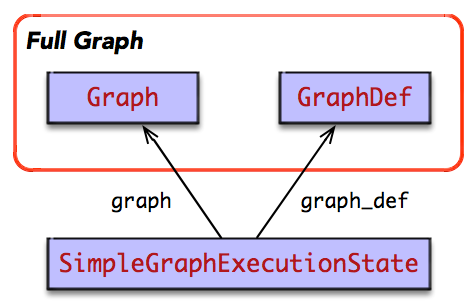
\includegraphics[width=0.5\textwidth]{figures/local-simple-graph-execution-state-model.png}
\caption{创建SimpleGraphExecutionState实例}
 \label{fig:local-simple-graph-execution-state-model}
\end{figure}

其中,\code{SimpleGraphExecutionState}的主要职责包括:

\begin{enum}
  \eitem{构造\code{FullGraph}}:发生在\code{DirectSession.Create};
  \eitem{执行简单的\ascii{OP}编排算法}:发生在\code{DirectSession.Create};
  \eitem{执行图的剪枝操作}:发生在\code{DirectSession.Run}。
\end{enum}

当执行\code{DirectSession::Create}时,将创建\code{SimpleGraphExecutionState}实例,并完成\code{FullGraph}实例的构建和初始化。

\begin{leftbar}
\begin{c++}
Status SimpleGraphExecutionState::MakeForBaseGraph(
    GraphDef* graph_def, const SimpleGraphExecutionStateOptions& opts,
    std::unique_ptr<SimpleGraphExecutionState>* out_state) {
  auto ret = std::make_unique<SimpleGraphExecutionState>(graph_def, opts));

  AddDefaultAttrsToGraphDef(&ret->original_graph_def_, *ret->flib_def_, 0));
  if (!ret->session_options_->config.graph_options().place_pruned_graph()) {
    ret->InitBaseGraph();
  }
  *out_state = std::move(ret);
  return Status::OK();
}
\end{c++}
\end{leftbar}

其中,\code{SimpleGraphExecutionState::InitBaseGraph}完成\code{FullGraph}从\code{GraphDef}到\code{Graph}的格式转换,并启动\code{SimplePlacer}的\ascii{OP}编排算法。

\begin{leftbar}
\begin{c++}
Status SimpleGraphExecutionState::InitBaseGraph() {
  auto ng = std::make_unique<Graph>(OpRegistry::Global());

  GraphConstructorOptions opts;
  ConvertGraphDefToGraph(opts, *original_graph_def_, ng.get());

  SimplePlacer placer(ng.get(), device_set_, session_options_);
  placer.Run();

  this->graph_ = ng.release();
  return Status::OK();
}
\end{c++}
\end{leftbar}

\subsubsection{图构造:GraphDef -> Graph}

刚开始,\code{SimpleGraphExecutionState}得到的是\code{GraphDef},这是最原始的图结构。它由\ascii{Client}将序列化后传递到后端\ascii{C++},然后由后端反序列化得到的图结构。

如\refig{local-graph-def-to-graph}所示,通过调用\code{ConvertGraphDefToGraph}将\code{GraphDef}实例变换为等价的\code{Graph}实例;同理,可以调用\code{Graph.ToGraphDef}将\code{Graph}实例变换为等价的\code{GraphDef}实例。

其中,\code{GraphDef}是使用\ascii{protobuf}格式存在的图结构,它包含了图所有元数据;而\code{Graph}则是运行时系统中用于描述图结构的领域对象,它不仅仅持有\code{GraphDef}的元数据,并包含其它图结构的其它信息。

\begin{figure}[H]
\centering
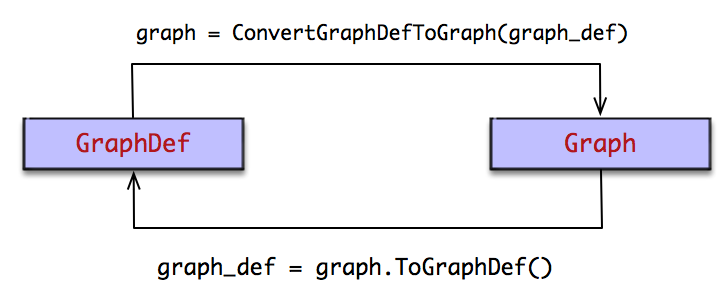
\includegraphics[width=0.6\textwidth]{figures/local-graph-def-to-graph.png}
\caption{\code{GraphDef}与\code{Graph}之间的格式转换}
 \label{fig:local-graph-def-to-graph}
\end{figure}

\subsubsection{OP编排:SimplePlacer}

\ascii{OP}的编排(\ascii{placement})指的是,将计算图中包含的\ascii{OP}以最高效的方式置放在合适的计算设备上运算,以最大化计算资源的利用率,可以形式化地描述为\refig{local-cost-model}。

\begin{figure}[H]
\centering
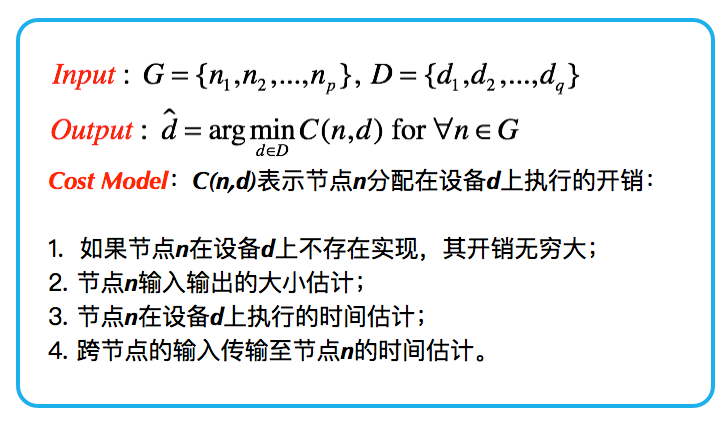
\includegraphics[width=0.6\textwidth]{figures/local-cost-model.png}
\caption{费用模型}
 \label{fig:local-cost-model}
\end{figure}

求取最优的编排方案,我猜想这是一个\ascii{NP}问题。该问题取决于计算图的特征,网络拓扑与带宽,样本数目等多个复杂的因素,该问题也是社区中最活跃的问题之一。

\subsection{迭代执行}

\code{DirectSession.Run}是\tf{}运行时的关键路径,它负责完成一次迭代计算。首先,\code{DirectSession}根据输入/输出对\code{FullGraph}实施剪枝,生成\code{ClientGraph};然后,根据所持有本地设备集,将\code{ClientGraph}分裂为多个\code{PartitionGraph};运行时为其每个\code{PartitionGraph}启动一个\code{Executor}实例,后者执行\code{PartitionGraph}的拓扑排序算法,完成计算图的执行。

具体实现,请参照\refsec{graph-operation-prune},\refsec{graph-operation-split},\refsec{graph-operation-exec}。

\subsubsection{图操作}

如\refig{local-graph-transformation}所示,在本地模式下,计算图经历三个形态的变换,最终被分解至各个计算设备上,以便实现在各个计算设备上并发执行子图。

\begin{figure}[H]
\centering
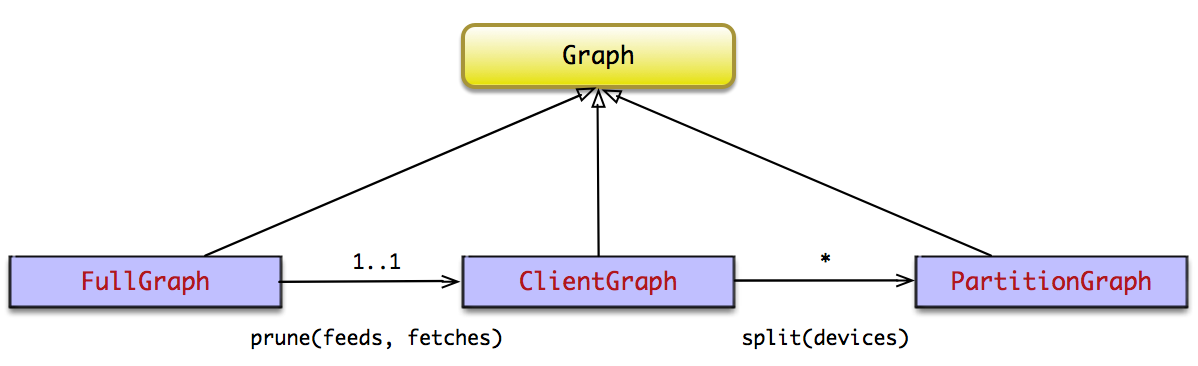
\includegraphics[width=0.9\textwidth]{figures/local-graph-transformation.png}
\caption{图变换}
 \label{fig:local-graph-transformation}
\end{figure}

\begin{itemize}
  \item \code{FullGraph}: \ascii{Client}负责构造的完整的计算图,常称为\code{FullGraph};但是,一次\code{Session.run}并不会执行整个计算图;
  \item \code{ClientGraph}: \ascii{Master}根据\code{Session.run}传递\code{feeds, fetches}输入输出列表,对\ascii{FullGraph}实施剪枝操作,计算得到本地迭代执行的最小依赖子图,常称为\code{ClientGraph};
  \item \code{PartitionGraph}: \ascii{Master}根据当前计算设备集,及其\ascii{OP}的设备约束规范,将\code{ClientGraph}分裂为多个\code{PartitionGraph};其中,每个计算设备对应一个\code{PartitionGraph},计算设备负责\code{PartitionGraph}的执行。
\end{itemize}

但是,\code{FullGraph, ClientGraph, PartitionGraph}的数据结构相同,它们都是\code{Graph}三种不同表现形式,仅仅大小和范畴存在差异。

\subsubsection{形式化}

在真实的系统实现中,本地模式的运行时是使用\ascii{C++}实现。其中,\tf{}运行时的关键路径为\code{run\_step}。因为真实系统实现中涉及过多的细节,不易发现算法的主干和逻辑。为了简化问题的描述,将形式化地描述\code{run\_step}的实现过程。

\begin{leftbar}
\begin{python}
def do_run_partitions(executors_and_partitions):
  barrier = ExecutorBarrier(executors_and_partitions.size())
  for (executor, partition) in executors_and_partitions:
    executor.run(partition, barrier)  
  barrier.wait()

def run_partitions(executors_and_partitions, inputs, outputs):
  frame = FunctionCallFrame()
  frame.set_args(inputs)
  do_run_partitions(executors_and_partitions)
  frame.get_ret_vals(outputs)

def run_step(devices, full_graph, inputs, outputs):
  client_graph = prune(full_graph, inputs, outputs)
  executors_and_partitions = split(client_graph, devices)
  run_partitions(executors_and_partitions, inputs, outputs)
\end{python}
\end{leftbar}

其中,在每个计算设备上,启动一个\code{Executor}执行分配给它的\code{PartitionGraph}。当某一个计算设备执行完所分配的\code{PartitionGraph}之后,\code{ExecutorBarrier}的计数器加\ascii{1},直至所有设备完成\code{PartitionGraph}列表的执行,\code{barrier.wait()}阻塞操作退出。

跨设备的\code{PartitionGraph}之间可能存在数据依赖关系,它们之间通过插入\code{Send/Recv}节点完成交互。事实上,在本地模式中,\code{Send/Recv}通过\code{Rendezvous}完成数据交换的。\code{Send}将数据放在\code{Rendezvous}上,而\code{Recv}则根据标识从\code{Rendezvous}取走。其中,\code{Send}不阻塞,而\code{Recv}是阻塞的。

\subsection{关闭会话}

\begin{leftbar}
\begin{c++}
Status DirectSession::Close() {
  cancellation_manager_->StartCancel();
  {
    mutex_lock l(closed_lock_);
    if (closed_) return Status::OK();
    closed_ = true;
  }
  return Status::OK();
}
\end{c++}
\end{leftbar}

如\refig{local-cancellation-manager}所示,将\ascii{Step}注册给\code{DirectSession}的\code{CancellationManager}之中。当\code{DirectSession}被关闭时,\code{DirectSession}的\code{CancellationManager},将取消这次\ascii{step}的执行过程。

\begin{figure}[H]
\centering
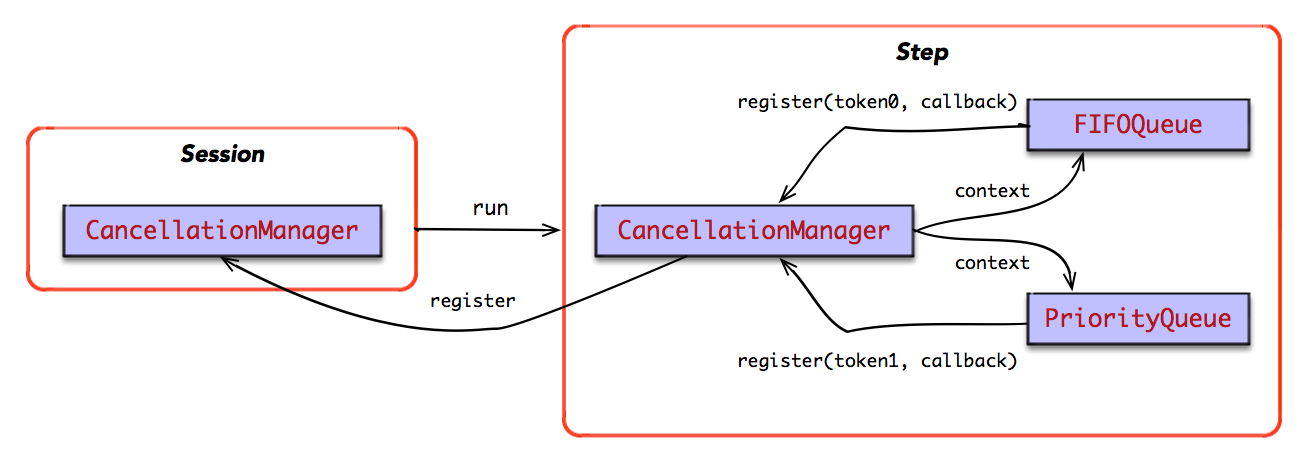
\includegraphics[width=0.9\textwidth]{figures/local-cancellation-manager.png}
\caption{CancellationManager工作原理}
 \label{fig:local-cancellation-manager}
\end{figure}

\begin{leftbar}
\begin{c++}
Status DirectSession::Run(
   const NamedTensorList& inputs,
   const std::vector<string>& output_names,
   const std::vector<string>& target_nodes,
   std::vector<Tensor>* outputs) {
  // step\_cancellation\_manager is passed to `OpKernelContext`
  CancellationManager step_cancellation_manager;

  // Register this step with session's cancellation manager, so that
  // `Session::Close()` will cancel the step.
  CancellationToken cancellation_token =
      cancellation_manager_->get_cancellation_token();
  bool already_cancelled = !cancellation_manager_->RegisterCallback(
      cancellation_token, [&step_cancellation_manager]() {
        step_cancellation_manager.StartCancel();
      });
  // ignore others...
}
\end{c++}
\end{leftbar}

当前\ascii{Step}的\code{CancellationManager}最终会传递给\code{OpKernelContext}。\ascii{Kernel}实现计算时,如果保存了中间状态,可以向其注册相应的回调钩子。其中,每个回调钩子都有唯一的\code{token}标识。

当\ascii{Step}被取消时,回调钩子被调用,该\ascii{Kernel}可以取消该\ascii{OP}的计算。例如,\code{FIFOQueue}实现\code{TryEnqueue}时,便往本次\ascii{Step}的\code{CancellationManager}注册了回调钩子,用于取消该\ascii{Kernel}中间的状态信息。

\begin{leftbar}
\begin{c++}
void FIFOQueue::TryEnqueue(const Tuple& tuple, OpKernelContext* ctx,
                           DoneCallback callback) {
  CancellationManager* cm = ctx->cancellation_manager();
  CancellationToken token = cm->get_cancellation_token();
  bool already_cancelled;
  {
    mutex_lock l(mu_);
    already_cancelled = !cm->RegisterCallback(
        token, [this, cm, token]() { Cancel(kEnqueue, cm, token); });
  }
  // ignore others...
}
\end{c++}
\end{leftbar}


\section{剪枝}
\label{sec:graph-operation-prune}

\code{DirectSession::Run}执行时,首先完成\code{ClientGraph}的构造。事实上,\code{ClientGraph}的构造过程,主要完成\code{FullGraph}的剪枝算法,并生成\code{ClientGraph}。

\subsection{构建ClientGraph}

如\refig{local-simple-graph-execution-state}所示,\code{SimpleGraphExecutionState}实例持有\code{FullGraph}实例,并根据输入/输出列表,生成\code{ClientGraph}。

\begin{figure}[H]
\centering
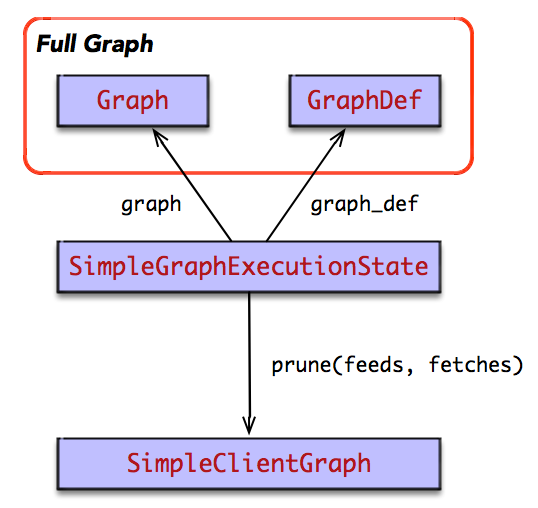
\includegraphics[width=0.55\textwidth]{figures/local-simple-graph-execution-state.png}
\caption{生成\code{ClientGraph}}
 \label{fig:local-simple-graph-execution-state}
\end{figure}

其中,\code{BuildGraphOptions}包含了输入/输出列表,调用\code{SimpleGraphExecutionState::BuildGraph}生成\code{ClientGraph}实例。

\begin{leftbar}
\begin{c++}
namespace {
  BuildGraphOptions build_graph_options(
    const NamedTensorList& inputs,
    const std::vector<string>& outputs,
    const std::vector<string>& targets) {
    // sort inputs/outputs/targets
    std::vector<string> inputs_sorted(inputs.begin(), inputs.end());
    std::sort(inputs_sorted.begin(), inputs_sorted.end());

    std::vector<string> outputs_sorted(outputs.begin(), outputs.end());
    std::sort(outputs_sorted.begin(), outputs_sorted.end());

    std::vector<string> tn_sorted(targets.begin(), targets.end());
    std::sort(tn_sorted.begin(), tn_sorted.end());

    // build graph options
    BuildGraphOptions options;
    options.feed_endpoints = inputs_sorted;
    options.fetch_endpoints = outputs_sorted;
    options.target_nodes = tn_sorted;
    options.use_function_convention = !run_state_args->is_partial_run;
    return options;
  }
}

Status DirectSession::Run(
  const RunOptions& run_options,
  const NamedTensorList& inputs,
  const std::vector<string>& output_names,
  const std::vector<string>& target_nodes,
  std::vector<Tensor>* outputs,
  RunMetadata* run_metadata) {

  // 1. prune graph
  // client\_graph = prune(full\_graph, inputs, outputs)
  std::unique_ptr<SimpleClientGraph> client_graph;
  execution_state_->BuildGraph(
    build_graph_options(inputs, output_names, target_nodes), 
    &client_graph);
   
  // 2. split graph into partition by devices 
  // executors\_and\_partitions = split(client\_graph, devices)
  
  // 3. lauch executor per partition
  // def run\_partitions(executors\_and\_partitions, inputs, outputs):
  // \ \ frame = FunctionCallFrame()
  // \ \ frame.set\_args(inputs)
  // \ \ for (executor, partition) in executors\_and\_partitions: 
  // \ \ \ \ exec.run(part)
  // \ \ frame.get\_ret\_vals(outputs)

  return Status::OK();
}
\end{c++}
\end{leftbar}

\code{ClientGraph}初始来自原始的\code{FullGraph},调用\code{RewriteGraphForExecution}函数,将根据输入/输出,对\code{ClientGraph}实施改写操作,包括增加节点,或删除节点,最终生成\code{SimpleClientGraph}实例。

\begin{leftbar}
\begin{c++}
const DeviceAttributes& 
SimpleGraphExecutionState::local_device_attr() const {
  return device_set_->client_device()->attributes();
}

Status SimpleGraphExecutionState::BuildGraph(
  const BuildGraphOptions& options, 
  std::unique_ptr<SimpleClientGraph>* out) {
  // 1. create new\_graph from origin graph, 
  // which is client graph.
  std::unique_ptr<Graph> ng;
  ng.reset(new Graph(flib_def_.get()));
  CopyGraph(*graph_, ng.get());

  // 2. prune the client graph
  subgraph::RewriteGraphForExecution(
    ng.get(), options.feed_endpoints, options.fetch_endpoints,
    options.target_nodes, local_device_attr(),
    options.use_function_convention);
  }

  // 3. create SimpleClientGraph, and return it.
  std::unique_ptr<SimpleClientGraph> dense_copy(
      new SimpleClientGraph(std::move(flib)));
  CopyGraph(*ng, &dense_copy->graph);
  *out = std::move(dense_copy);

  return Status::OK();
}
\end{c++}
\end{leftbar}

因此,构建\code{ClientGraph}过程,其关键路径为\code{RewriteGraphForExecution},即剪枝算法。剪枝算法根据输入/输出列表,反向遍历\ascii{FullGraph},找到最小的依赖子图\code{ClientGraph}。

一般地,对于\code{ClientGraph}输入节点,扮演了起始节点;而输出节点,扮演了终止节点。因此,关于输入和输出,存在两个比较棘手的问题:

\begin{enum}
  \eitem{输入:当\code{ClientGraph}计算开始前,外部的运行时如何传递\code{Tensor}给输入节点};
  \eitem{输出:当\code{ClientGraph}计算完成后,外部的运行时又如何从输出节点获取\code{Tensor}}。
\end{enum}

存在两种媒介:\code{FunctionCallFrame}和\code{Rendezvous},外部运行时与输入/输出节点可以使用其中一种媒介交换数据。

\code{FunctionCallFrame}用于\code{Arg/RetVal}函数调用的\ascii{OP},用于函数调用时传递函数参数值,及其返回函数值。但是,它们仅适用于单进程的运行时环境。

\code{Rendezvous}用于\code{Send/Recv}消息发送的\ascii{OP},这是一种更为通用的通信方式,适用于分布式的运行时环境。

\subsection{基于Rendezvous}

如\refig{client-prune-graph}所示,根据\code{fetches}列表,反向搜索依赖的节点,直至\code{feeds},计算得到最小依赖的子图。

对于\code{Feed}的边实施剪枝,例如剪枝\code{ina:0})边,并在此处插入节点\code{Recv},并按照输入边的名字命名该节点,例如\code{\_recv\_ina\_0}。

同理,对于\code{Fetch}的边也实施剪枝,例如剪枝\code{f:0}边,并在此处插入节点\code{Send}节点,并按照输出边的名字命名该节点,例如\code{\_send\_f\_0}。

最终,通过插入\code{Source/Sink}节点,将剪枝后得到各个联通的子图进行汇总,形成一个完整的\ascii{DAG}图。

\begin{figure}[H]
\centering
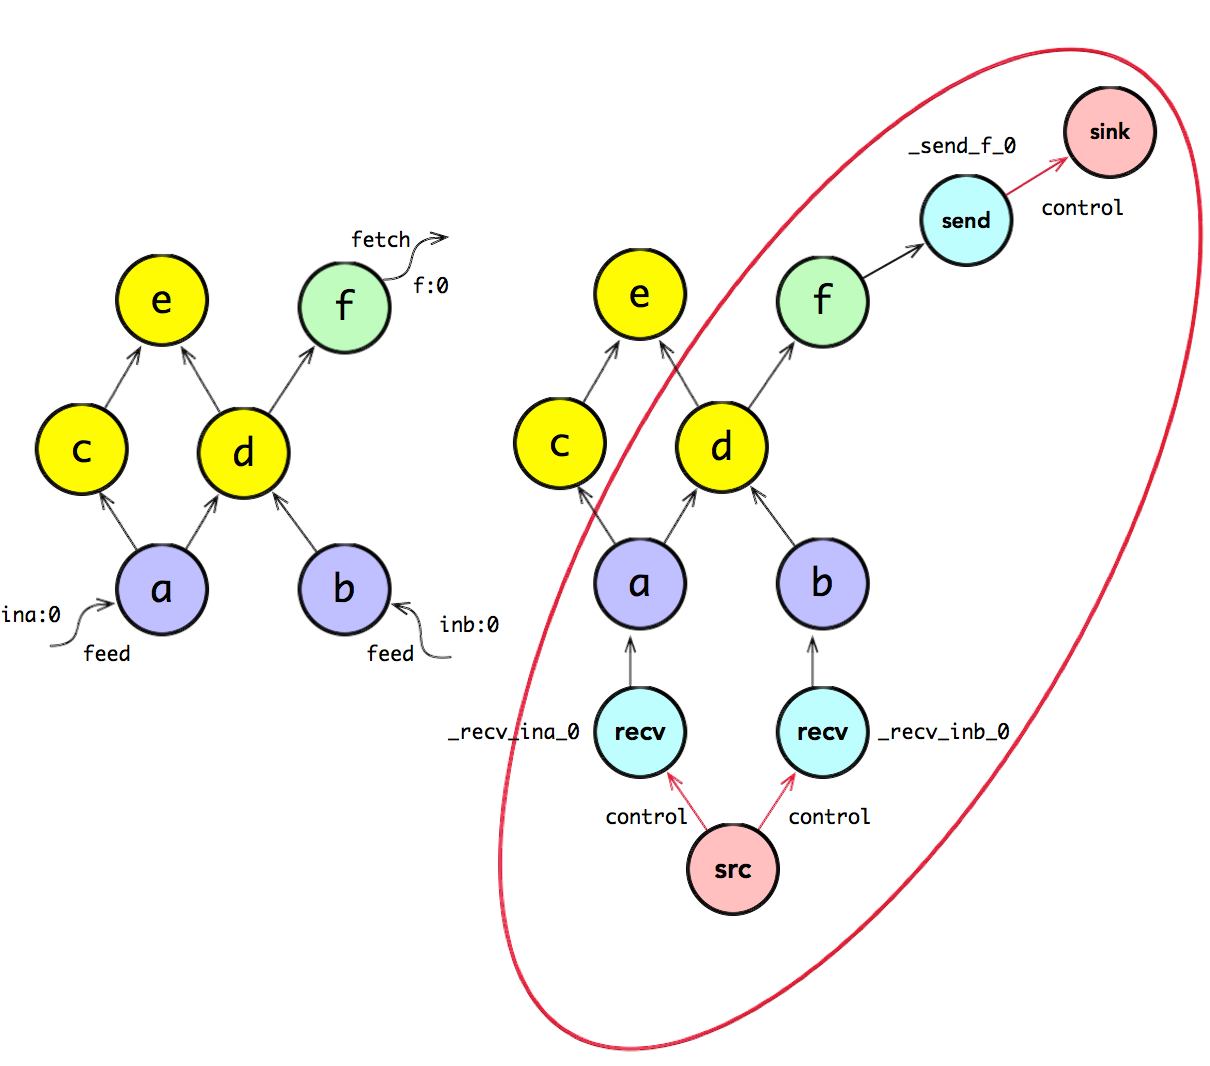
\includegraphics[width=0.9\textwidth]{figures/client-prune-graph.png}
\caption{图剪枝:插入Send/Recv节点}
 \label{fig:client-prune-graph}
\end{figure}

\subsection{基于FunctionCallFrame}

但是,输入/输出通过\code{Rendezvous}交换数据可能存在性能上的瓶颈。因为待发送的\code{Tensor}需要携带发送设备,接收设备,\code{TensorId},共同组成了唯一的字符串标识,数据发送和接收需要花费很长的字符串解析的时间开销。

特殊地,对于本地模式,因为在同一进程内,使用\code{Rendezvous}交换数据存在不必要的性能损耗。可以使用基于\code{FunctionCallFrame}函数调用替代之。

因此,在本地模式下,可以使用\code{Arg/RetVal}分别替代\code{Send/Recv}节点,从而实现了函数调用交换数据的方式,替代原有基于\code{Rendezvous}交互数据的方式。

如\refig{client-prune-graph-function-ops}所示。对于\code{Feed}的边实施剪枝,例如剪枝\code{ina:0})边,并在此处插入节点\code{Arg},并按照输入边的名字命名该节点,例如\code{\_arg\_ina\_0}。

同理,对于\code{Fetch}的边也实施剪枝,例如剪枝\code{f:0}边,并在此处插入节点\code{RetVal}节点,并按照输出边的名字命名该节点,例如\code{\_retval\_f\_0}。

最终,通过插入\code{Source/Sink}节点,将剪枝后得到各个联通的子图进行汇总,形成一个完整的\ascii{DAG}图。

\begin{figure}[H]
\centering
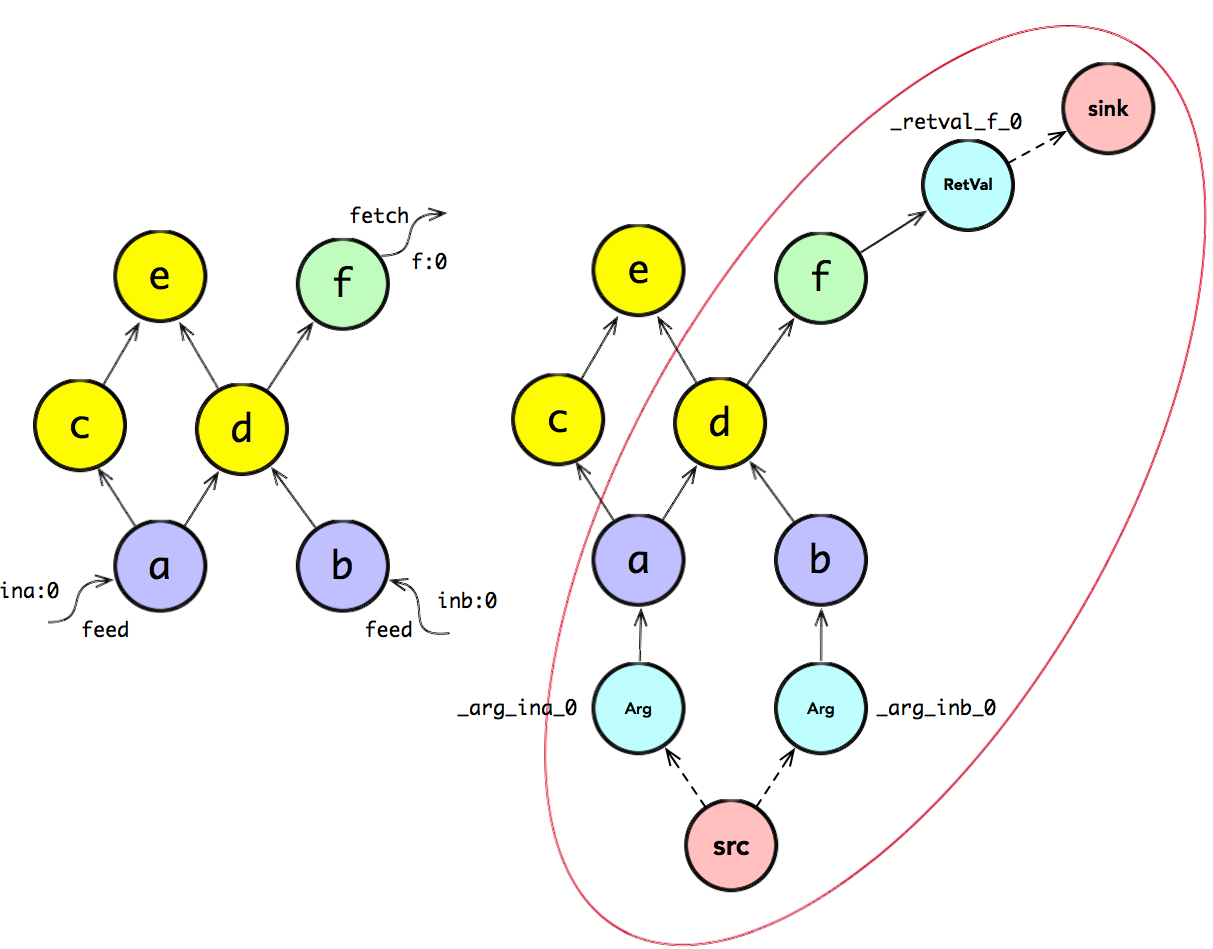
\includegraphics[width=0.9\textwidth]{figures/client-prune-graph-function-ops.png}
\caption{图剪枝:插入Arg/RetVal节点}
 \label{fig:client-prune-graph-function-ops}
\end{figure}

\subsection{剪枝算法实现}

剪枝算法主要由\code{RewriteGraphForExecution}完成,主要包括\ascii{3}个子过程。

\begin{enum}
  \eitem{追加输入节点}
  \eitem{追加输出节点} 
  \eitem{反向剪枝}
\end{enum}

\begin{leftbar}
\begin{c++}
void RewriteGraphForExecution(Graph* g, bool use_function, 
    const ArraySlice<string>& fed_outputs,
    const ArraySlice<string>& fetch_outputs,
    const ArraySlice<string>& target_node_names,
    const DeviceAttributes& device_info) {
  FeedInputs(g, use_function, device_info, fed_outputs);

  std::vector<Node*> fetch_nodes;
  FetchOutputs(g, use_function, device_info, 
    fetch_outputs, &fetch_nodes);

  PruneForTargets(g, fetch_nodes, target_node_names);
}
\end{c++}
\end{leftbar}

\subsubsection{追加输入节点}

如\refig{local-prune-feed}所示,对于任意一条输入边实施剪枝时,插入相应的\code{Arg}或\code{Recv}节点,删除既有的边,并重新连接相应的边。

在计算图中,一条边唯一地由\code{TensorId}标识,它由\code{op:src\_output}二元组构成。前者表示边的上游节点,后者表示给边为上游节点的第几条边。

示例代码删除了部分不重要的逻辑,并搬迁了部分函数的职责,并在局部尝试部分函数提取,以便更好地还原算法的逻辑。其中,假设\code{Graph}可以按照\code{TensorId}索引节点和边。

\begin{figure}[H]
\centering
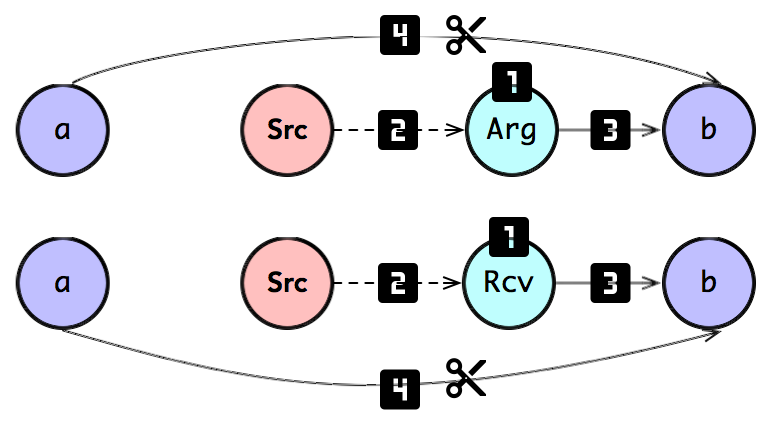
\includegraphics[width=0.6\textwidth]{figures/local-prune-feed.png}
\caption{剪枝:输入边}
 \label{fig:local-prune-feed}
\end{figure}

\begin{leftbar}
\begin{c++}
namespace {
  DataType data_type(Graph& g, const TensorId& tensor_id) {
    Node* upstream_node = g.upstream_node(tensor_id);
    return BaseType(upstream_node->output_type(tensor_id.src_output()));
  }

  Node* AppendRecvNode(Graph& g, 
    const TensorId& tensor_id, const DeviceAttributes& device_info) {
      Node* recv_node;
      NodeBuilder(strings::StrCat(
        "_recv_", tensor_id.op(), "_", tensor_id.src_output()), "_Recv")
        .Attr("tensor_type", data_type(g, tensor_id))
        .Attr("tensor_name", tensor_id.name())
        .Attr("send_device", device_info.name())
        .Attr("recv_device", device_info.name())
        .Attr("send_device_incarnation", device_info.incarnation())
        .Attr("client_terminated", true)
        .Finalize(g, &recv_node);
      return recv_node;
  }

  Node* AppendArgNode(Graph& g, size_t index, 
    const TensorId& tensor_id, const DeviceAttributes& device_info) {
    Node* arg_node;
    NodeBuilder(strings::StrCat(
      "_arg_", tensor_id.op(), "_", tensor_id.src_output()), "_Arg")
      .Attr("T", data_type(g, tensor_id))
      .Attr("index", index)
      .Finalize(g, &arg_node);
    return arg_node;
  }

  // 1. append arg/recv node
  Node* AppendNewNode(Graph& g, bool use_function, size_t index, 
    const TensorId& tensor_id,const DeviceAttributes& device_info) {
    if (use_function) {
      return AppendArgNode(g, index, tensor_id, device_info);
    } else {
      return AppendRecvNode(g, tensor_id, device_info);
    }
  }

  void AppendNewEdges(Graph& g, 
    Node* new_node, const TensorId& tensor_id) {
    // 2. add control edge between source node and new node.
    g.AddControlEdge(g.source_node(), new_node);

    Edge* old_edge = g.edge(tensor_id);
    
    // 3. add edge between new node and downstream node.
    g.AddEdge(new_node, 0, old_edge->dst(), old_edge->dst_input());
    
    // 4. remove old edge.
    g.RemoveEdge(old_edge);
  }
}

void FeedInputs(Graph& g, bool use_function,
  const DeviceAttributes& device_info,
  const ArraySlice<TensorId>& feeds) {
  for (size_t i = 0; i < feeds.size(); ++i) {
    Node* new_node = AppendNewNode(use_function, i, feeds[i]);
    AppendNewEdges(g, new_node, feeds[i]);
  }
}
\end{c++}
\end{leftbar}

\subsubsection{追加输出节点}

对于任意一条输出边实施剪枝时,插入相应的\code{RetVal}或\code{Send}节点,并将其与\code{Sink}节点通过控制依赖边连接。

如\refig{local-prune-fetch}所示,对输出边实施剪枝操作。新节点与上游节点的连接关系,在构造新节点时,通过\code{Input}已经指定。另外,函数直接返回了新节点(\code{RetVal/Send})为终止节点,因此没必要删除原来的边,其算法与输入边的处理存在微妙的差异。

\begin{figure}[H]
\centering
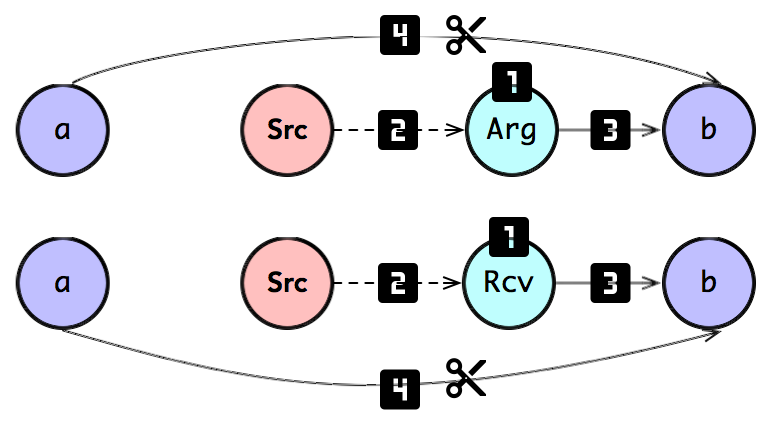
\includegraphics[width=0.6\textwidth]{figures/local-prune-feed.png}
\caption{剪枝:输出边}
 \label{fig:local-prune-fetch}
\end{figure}

\begin{leftbar}
\begin{c++}
namespace {
  Node* AppendSendNode(Graph& g, 
    const TensorId& tensor_id, const DeviceAttributes& device_info) {
    Node* send_node;
    NodeBuilder(strings::StrCat(
      "_send_", tensor_id.op(), "_", id.src_output()), "_Send")
      // 2. add edge between upstream node and send node.
      .Input(g.upstream_node(tensor_id), tensor_id.src_output())
      .Attr("tensor_name", tensor_id.name())
      .Attr("send_device", device_info.name())
      .Attr("recv_device", device_info.name())
      .Attr("send_device_incarnation",
            device_info.incarnation())
      .Attr("client_terminated", true)
      .Finalize(g, &send_node);
    return send_node;
  }

  Node* AppendRetvalNode(Graph& g, size_t index, 
    const TensorId& tensor_id, const DeviceAttributes& device_info) {
    Node* retval_node;
    NodeBuilder(strings::StrCat(
      "_retval_", tensor_id.op(), "_", tensor_id.src_output(), "_", index), 
      "_Retval")
      // 2. add edge between upstream node and retval node.
      .Input(g.upstream_node(tensor_id), tensor_id.src_output())
      .Attr("T", data_type(g, tensor_id))
      .Attr("index", index)
      .Finalize(g, &retval_node))
    return retval_node;
  }

  // 1. append retval/send node
  Node* AppendNewNode(Graph& g, bool use_function, size_t index, 
    const TensorId& tensor_id,const DeviceAttributes& device_info) {
    if (use_function) {
      return AppendRetvalNode(g, index, tensor_id, device_info);
    } else {
      return AppendSendNode(g, tensor_id, device_info);
    }
  }
}

void FetchOutputs(Graph& g, bool use_function,
  const DeviceAttributes& device_info,
  const ArraySlice<TensorId>& fetches,
  std::vector<Node*>& fetch_nodes) {
  for (size_t i = 0; i < fetches.size(); ++i) {
    Node* new_node = AppendNewNode(use_function, i, fetches[i]);
    
    // 3. add control edge between new node and sink node. 
    g->AddControlEdge(new_node, g->sink_node());

    fetch_nodes.push_back(new_node);
  }
}
\end{c++}
\end{leftbar}

\subsubsection{反向剪枝}

剪枝操作,其本质就是\ascii{DAG}反向的宽度优先遍历算法。首先,创建了一个队列,及其一个\code{visited}数组,后者用于记录已经遍历过的节点。初始化时,队列仅包含输出节点和输入节点(\code{targets})。当图遍历完毕后,不再\code{visited}里面的节点,表示本此执行不依赖于它,应从图中删除该节点,及其相关联的边。

经过剪枝后,将形成若干\ascii{DAG}子图。将入度为\code{0}的节点,与\code{Source}节点通过控制依赖边相连接;出度为\ascii{0}的节点,与\code{Sink}节点通过控制依赖边相连接,最终形成一个完整的\ascii{DAG}图。

\begin{leftbar}
\begin{c++}
namespace {
  void ReverseBFS(
    Graph* g, std::unordered_set<const Node*>& visited) {
    std::deque<const Node*> queue(visited.begin(), visited.end());
    while (!queue.empty()) {
      const Node* n = queue.front();
      queue.pop_front();
      for (const Node* in : n->in_nodes()) {
        if (visited.insert(in).second) {
          queue.push_back(in);
        }
      }
    }
  }

  void RemoveUnvisitedNodes(
    Graph* g, std::unordered_set<const Node*>& visited) {
    for (Node* n : g->nodes()) {
      if (visited.count(n) == 0 && !n->IsSource() && !n->IsSink()) {
        g->RemoveNode(n);
      }
    }
  }

  void PruneForReverseReachability(
    Graph* g, std::unordered_set<const Node*>& visited) {
    ReverseBFS(g, visited);
    RemoveUnvisitedNodes(g, visited);
  }

  void FixupSourceEdges(Graph* g, Node* n) {
    if (!n->IsSource() && n->in_edges().empty()) {
      g->AddControlEdge(g->source_node(), n);
    }  
  }

  void FixupSinkEdges(Graph* g, Node* n) {
    if (!n->IsSink() && n->out_edges().empty()) {
      g->AddControlEdge(n, g->sink_node());
    }  
  }

  void FixupSourceAndSinkEdges(Graph* g) {
    for (Node* n : g->nodes()) {
      FixupSourceEdges(g, n);
      FixupSinkEdges(g, n);
    }
  }

  void AppendTargetNodes(Graph& g, 
    const ArraySlice<string>& target_names,
    std::unordered_set<const Node*>& targets) {
    for (auto name : target_names) {
      Node* target = g.GetNodeBy(name);
      targets.insert(target);
    }
  }  
}

void PruneForTargets(Graph* g, 
  std::vector<Node*>& fetch_nodes,
  const ArraySlice<string>& target_names) {
  std::unordered_set<const Node*> targets(
    begin(fetch_nodes), end(fetch_nodes));

  AppendTargetNodes(g, target_names, targets);
  PruneForReverseReachability(g, targets);
  FixupSourceAndSinkEdges(g);
}
\end{c++}
\end{leftbar}

\section{分裂}
\label{sec:graph-operation-split}

如\refig{local-graph-split-by-device}所示,假如\code{d}节点放置在\ascii{GPU0}上执行,而其他节点放置在\ascii{CPU0}上执行。其中,节点\code{a}与\code{b}通过\code{Arg}输入数据;节点\code{f}将其结果输出到\code{RetVal}节点上。

\begin{figure}[H]
\centering
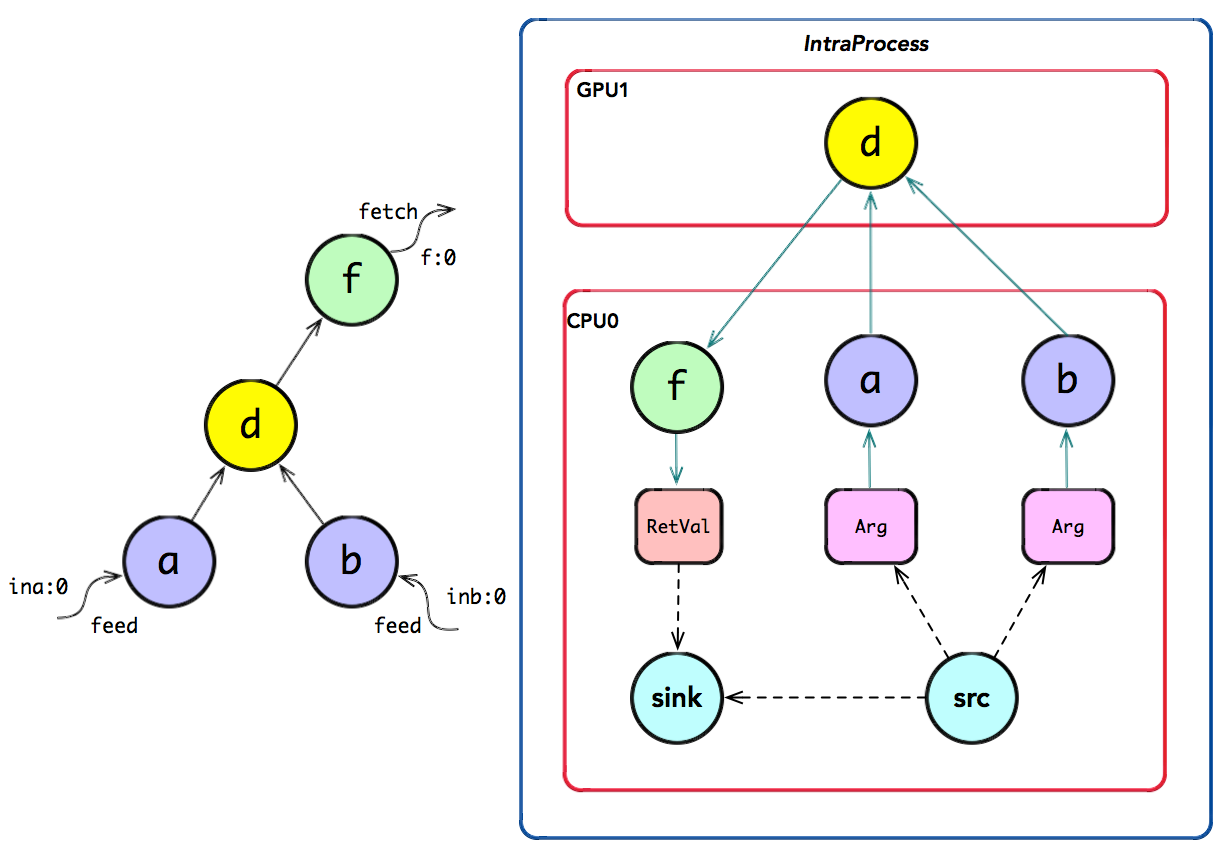
\includegraphics[width=0.9\textwidth]{figures/local-graph-split-by-device.png}
\caption{按本地设备集执行图分裂}
 \label{fig:local-graph-split-by-device}
\end{figure}

因此,计算图中存在若干条边跨越设备。对于跨越设备的边,运行时将其分裂,并就地插入\code{Send/Recv}边,分别用于原设备上发送数据,并在目标设备上接受数据,完成设备间的数据交换。如\refig{local-graph-split-insert-send-recv}所示。

其中,\code{Arg/RetVal}节点通过媒介\code{FunctionCallFrame}交换数据;\code{Send/Recv}节点通过媒介\code{Rendezvous}交换数据。

\begin{figure}[H]
\centering
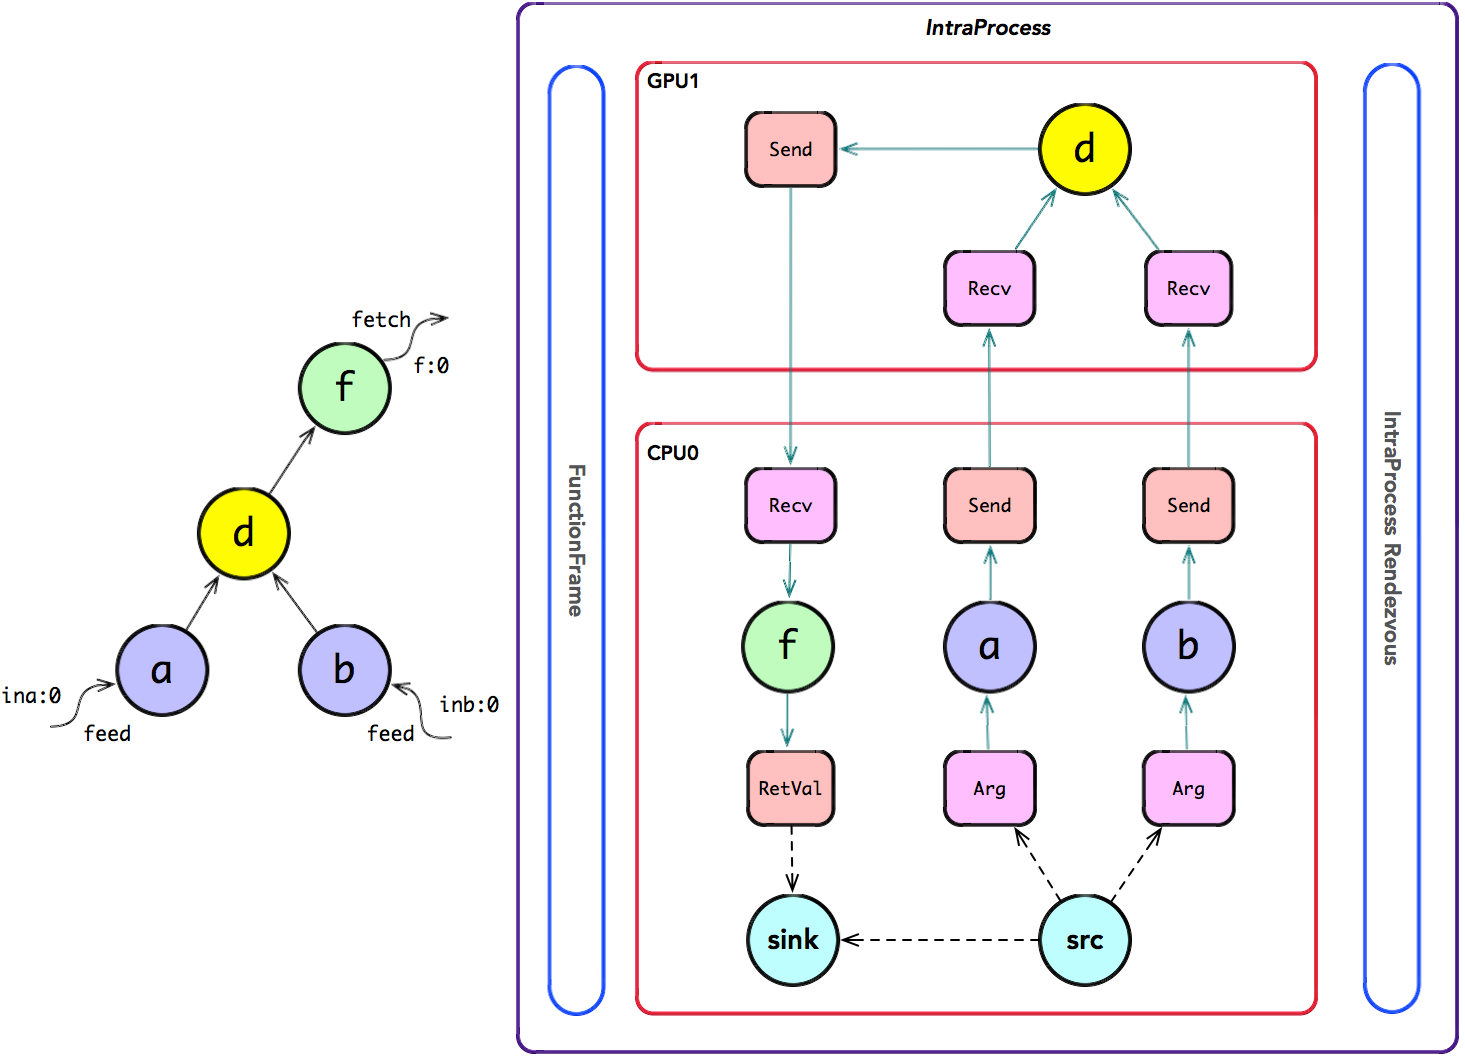
\includegraphics[width=1.0\textwidth]{figures/local-graph-split-insert-send-recv.png}
\caption{跨设备OP之间插入Send/Recv节点}
 \label{fig:local-graph-split-insert-send-recv}
\end{figure}

\subsection{情况1}

最简单的情况下,\code{src}与\code{dst}在同一个\code{Partition}内。因此,直接将其划归在同一个\code{Partition}即可。

\begin{figure}[H]
\centering
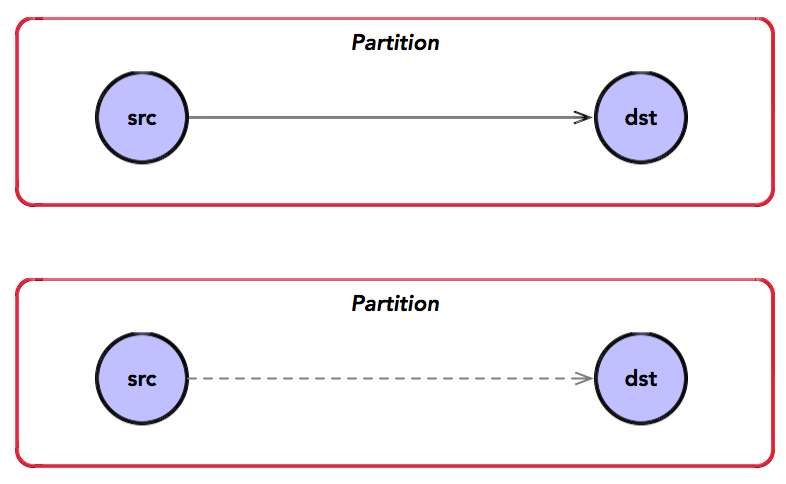
\includegraphics[width=0.6\textwidth]{figures/split-graph-1.png}
\caption{情况1:src与dst在同一个Partition内}
 \label{fig:split-graph-1}
\end{figure}

\subsection{情况2}

如果\code{src}与\code{dst}不在同一个\code{Partition}内,但两者之间原来是通过普通边连接在一起的。因此,仅需要在它们中间增加\code{Send}与\code{Recv}节点,将其划归在两个不同的\code{Partition}内。

\begin{figure}[H]
\centering
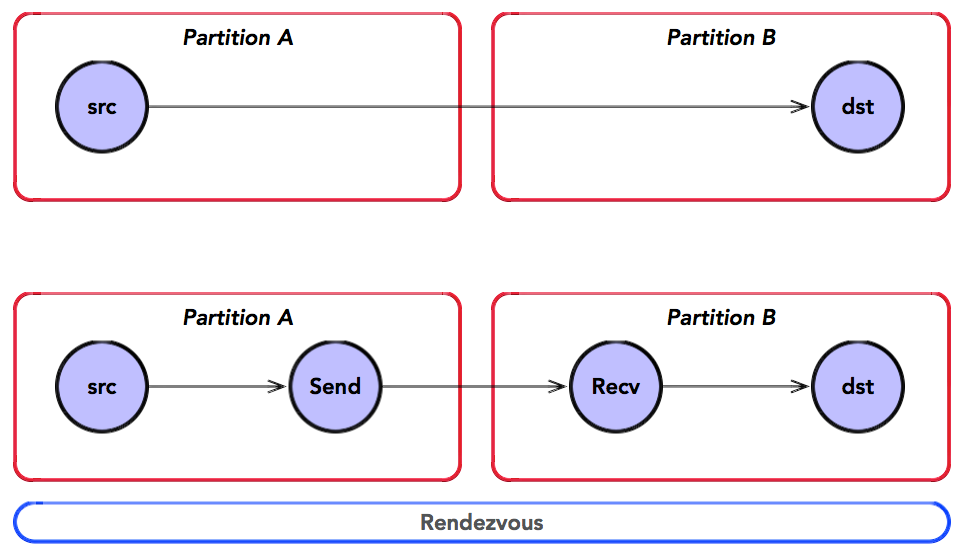
\includegraphics[width=0.7\textwidth]{figures/split-graph-2.png}
\caption{情况2:src与dst不在同一个Partition内,但两者之间是普通边}
 \label{fig:split-graph-2}
\end{figure}

\subsection{情况3}

如果\code{src}与\code{dst}不在同一个\code{Partition}内,但两者之间原来是通过控制依赖边连接在一起的。

此时,需要在\code{src}侧增加一个\code{Const}的\code{DummyNode},并作为\code{src}的下游通过控制依赖边相连;最终,在通过\code{Send}将其值发送到对端。

在\code{dst}侧,\code{Recv}收到该值,使用\code{Identity}将其消费掉;最终,再将\code{Identity}与\code{dst}连接控制依赖边。

在这里,\code{Const}扮演生产者,\code{Identity}扮演消费者角色。既满足了跨设备间通信的需求,又满足原来\code{src}与\code{dst}之间的控制依赖的关系。但是,其缺点就是存在微妙的性能开销。

\begin{figure}[H]
\centering
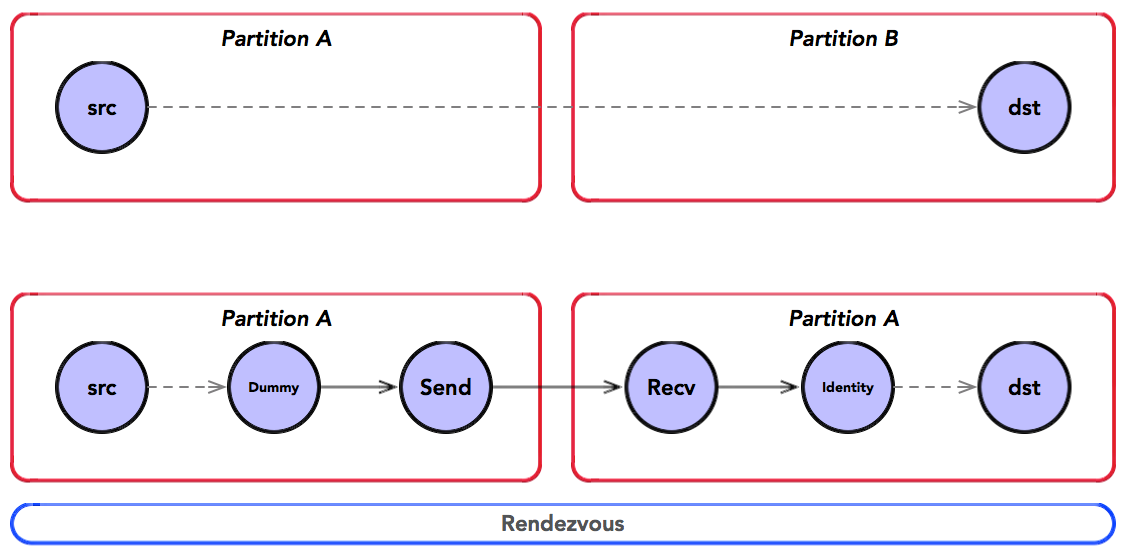
\includegraphics[width=0.8\textwidth]{figures/split-graph-3.png}
\caption{情况3:src与dst不在同一个Partition内,但两者之间是控制依赖边}
 \label{fig:split-graph-3}
\end{figure}

\subsection{分裂算法实现}

分裂算法也是一个反向遍历图的算法。对于当前遍历的节点,将其标记为\code{dst};然后再寻找\code{dst}的所有输入边;遍历所有输入边,从而找到与改边相连的源节点,将其标记为\code{src}。

因此,更具上述讨论的三种情况,迭代实现\code{src}与\code{dst}两者之前的\code{Partition}划分算法。

\begin{leftbar}
\begin{c++}
namespace {
  
  using Edges = std::vector<const Edge*>;
  using Partitions = std::unordered_map<string, GraphDef>;

  void AddInput(NodeDef* dst, StringPiece src_name, int src_slot) {
    if (src_slot == Graph::kControlSlot) {
      dst->add_input(strings::StrCat("^", src_name));
    } else if (src_slot == 0) {
      dst->add_input(src_name.data(), src_name.size());
    } else {
      dst->add_input(strings::StrCat(src_name, ":", src_slot));
    }
  }

  Edges InputsOf(const Node* dst) {
    Edges inputs(dst->num_inputs(), nullptr);
    for (auto edge : dst.in_edges()) {
      if (edge->IsControlEdge()) {
        inputs.push_back(e);
      } else {
        inputs[edge->dst_input()] = edge;
      }
    }
    return inputs;
  }

  NodeDef* InitDstNodeDef(const Node& dst, NodeDef* dst_def) {
    dst_def = dst.def();
    dst_def->set_device(dst.assigned_device_name());
    dst_def->clear_input();
    return dst_def;  
  }

  NodeDef* AddDummyConst(const PartitionOptions& opts, GraphDef* gdef,
                         const Edge* edge, Status* status) {
    const Node* src = edge->src();
    Tensor tensor(DT_FLOAT, TensorShape({0}));
    NodeDef* result = gdef->add_node();
    *status = NodeDefBuilder(opts.new_name(src->name()), "Const")
                  .Device(src->assigned_device_name())
                  .Attr("dtype", DT_FLOAT)
                  .Attr("value", tensor)
                  .Finalize(result);
    return result;
  }

  NodeDefBuilder::NodeOut BuildSendFrom(
      const PartitionOptions& opts,
      GraphDef* src_graph,
      const Edge* edge,
      NodeDefBuilder::NodeOut& send_from) {
    if (edge->IsControlEdge()) {
      // Case 3: DummyNode(Const) -ctrl-> src -> send  
      NodeDef* dummy = AddDummyConst(opts, src_graph, edge);
      AddInput(dummy, edge->src()->name(), Graph::kControlSlot);
      send_from.Reset(dummy->name(), 0, DT_FLOAT);
    } else {
      // Case 2: src -> send  
      send_from.Reset(edge->src()->name(),
                      edge->src_output(), 
                      EdgeType(edge));
    }
  }

  void SetSendRecvAttrs(
      const PartitionOptions& opts, 
      const Edge* edge,
      NodeDefBuilder* builder) {
    builder->Attr("tensor_name",
                  strings::StrCat("edge_", edge->id(), "_", edge->src()->name()));
    builder->Attr("send_device", edge->src()->assigned_device_name());
    builder->Attr("send_device_incarnation",
                  static_cast<int64>(
                      opts.get_incarnation(edge->src()->assigned_device_name())));
    builder->Attr("recv_device", edge->dst()->assigned_device_name());
    builder->Attr("client_terminated", false);
  }

  NodeDef* AddSend(
      const PartitionOptions& opts, 
      GraphDef* gdef, 
      const Edge* edge,
      NodeDefBuilder::NodeOut send_from) {
    NodeDef* send = gdef->add_node();
    NodeDefBuilder builder(opts.new_name(edge->src()->name()), "_Send");
    SetSendRecvAttrs(opts, edge, &builder);
    builder.Device(edge->src()->assigned_device_name())
           .Input(send_from)
           .Finalize(send);
    return send;
  }

  NodeDef* AddRecv(const PartitionOptions& opts, const GraphInfo& g_info,
                   GraphDef* gdef, const Edge* edge, NodeDef** real_recv,
                   Status* status) {
    NodeDef* recv = gdef->add_node();
    NodeDefBuilder builder(opts.new_name(src->name()), "_Recv");
    SetSendRecvAttrs(opts, edge, &builder);
    builder.Device(dst->assigned_device_name())
           .Attr("tensor_type", EdgeType(edge))
           .Finalize(recv);
    return recv;

    if (edge->IsControlEdge()) {
      // Case 3: Recv -> Identity -contrl-> dst
      NodeDef* id = gdef->add_node();
      NodeDefBuilder(opts.new_name(src->name()), "Identity")
          .Device(dst->assigned_device_name())
          .Input(recv->name(), 0, cast_dtype)
          .Finalize(id);
      return id;
    } else {
      return recv;
    }
  }

  void InsertSendRecv(
      const PartitionOptions& opts,
      GraphDef* src_graph, 
      Edge* edge, 
      GraphDef* dst_graph, 
      NodeDef* dst_def) {
    NodeDefBuilder::NodeOut send_from;
    BuildSendFrom(opts, src_graph, edge, send_from);

    NodeDef* send = AddSend(opts, src_graph, edge, send_from);
    NodeDef* recv = AddRecv(opts, dst_graph, edge);

    if (edge->IsControlEdge()) {
      // Case 3: In fact, recv is identity.
      AddInput(dst_def, recv->name(), Graph::kControlSlot);
    } else {
      AddInput(dst_def, recv->name(), 0);
    }
  }
}

Status Partition(const PartitionOptions& opts, 
                 Partitions& partitions, Graph& client_graph) {
  for (const Node* dst : client_graph.op_nodes()) {
    // 1. find dst node
    GraphDef* dst_graph = &partitions[opts.node_to_loc(dst)];
    NodeDef* dst_def = InitDstNodeDef(*dst, dst_graph->add_node());
    
    // 2. search all input edges.
    for (const Edge* edge : InputsOf(dst)) {
      // 3. find src node: edge->src()
      GraphDef* src_graph = &partitions[opts.node_to_loc(src)];

      // skip sink/source nodes.
      if (!edge->src()->IsOp()) 
        continue;  

      // Case 1: same partition
      if (src_graph == dst_graph) {
        AddInput(dst_def, src->name(), edge->src_output());
        continue;
      }

      // Case 2-3: different partition
      InsertSendRecv(opts, src_graph, edge, dst_graph, dst_def);
    }
  }
}
\end{c++}
\end{leftbar}

\subsection{回调函数}

在\code{PartitionOptions}中,存在两个重要的回调函数。\code{NodeToLocFunc}用于图分裂;\code{NewNameFunc}用于给新增加的节点命名,例如\code{Send/Recv}。

\begin{leftbar}
\begin{c++}
struct PartitionOptions {
  typedef std::function<string(const Node*)> NodeToLocFunc;
  NodeToLocFunc node_to_loc = nullptr;

  typedef std::function<string(const string&)> NewNameFunc;
  NewNameFunc new_name = nullptr;

  // ignore others...
};
\end{c++}
\end{leftbar}

对于图分裂,存在两种最基本的分裂方法。

\begin{leftbar}
\begin{c++}
string SplitByDevice(const Node* node) {
  return node->assigned_device_name();
}

string SplitByWorker(const Node* node) {
  string task, device;
  DeviceNameUtils::SplitDeviceName(
      node->assigned_device_name(), &task, &device);
  return task;
}
\end{c++}
\end{leftbar}

在本地模式下,\code{NodeToLocFunc}被配置为\code{SplitByDevice}。如图\code{intraprocess-splity-by-device}所示。

\begin{figure}[H]
\centering
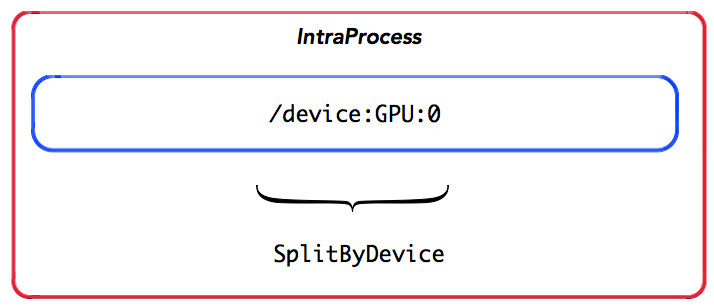
\includegraphics[width=0.7\textwidth]{figures/intraprocess-splity-by-device.png}
\caption{本地模式:SplitByDevice}
 \label{fig:intraprocess-splity-by-device}
\end{figure}


在分布式模式下,\code{Master}的\code{NodeToLocFunc}被配置为\code{SplitByWorker};而\code{Worker}
的\code{NodeToLocFunc}被配置为\code{SplitByDevice}。

因此,在分布式模式下,图分裂经历了两级分离。第一级按照\code{SplitByWorker}分裂,将图划分到各个\code{Worker}上去;第二级按照\code{SplitByDevice},再将图划分到各个计算设备上去。

\begin{figure}[H]
\centering
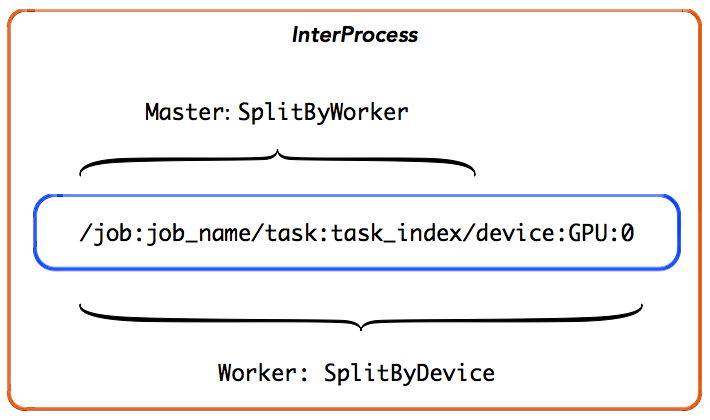
\includegraphics[width=0.7\textwidth]{figures/interprocess-splity-by-worker.png}
\caption{分布式模式:两级分裂}
 \label{fig:interprocess-splity-by-worker}
\end{figure}

\section{执行}
\label{sec:graph-operation-exec}

接下来,运行时将并发执行各个\code{PartitionGraph}。如\refig{local-graph-execution}所示,每个\code{PartitionGraph}启动一个\code{Executor},实现并发执行图的计算。

每个\code{Executor}将执行\code{PartitionGraph}的拓扑排序算法,将入度为\ascii{0}的\ascii{OP}追加到\code{ready\_queue}之中,并将其关联的\ascii{OP}的入度减\ascii{1}。调度器调度\code{ready\_queue}之中\ascii{OP
},并将其放入\code{ThreadPool}中执行对应的\ascii{Kernel}实现。

在所有\code{Partition}开始并发执行之前,需要外部将其输入传递给相应的\code{Arg}节点;当所有\code{Partition}完成计算后,外部再从\code{RetVal}节点中取走数据。其中,\code{Arg/RetVal}节点之间的数据时通过\code{FunctionCallFrame}完成交互的。

如果\code{PartitionGraph}之间需要跨设备交换数据,生产者将其放在\code{Send}节点,消费者通过\code{Recv}节点获取数据。其中,发送方不阻塞;接收方如果数据未到,则发生阻塞直至超时。此外,\code{Send/Recv}节点之间的数据是通过\code{Rendezvous}完成交互的。

\begin{figure}[H]
\centering
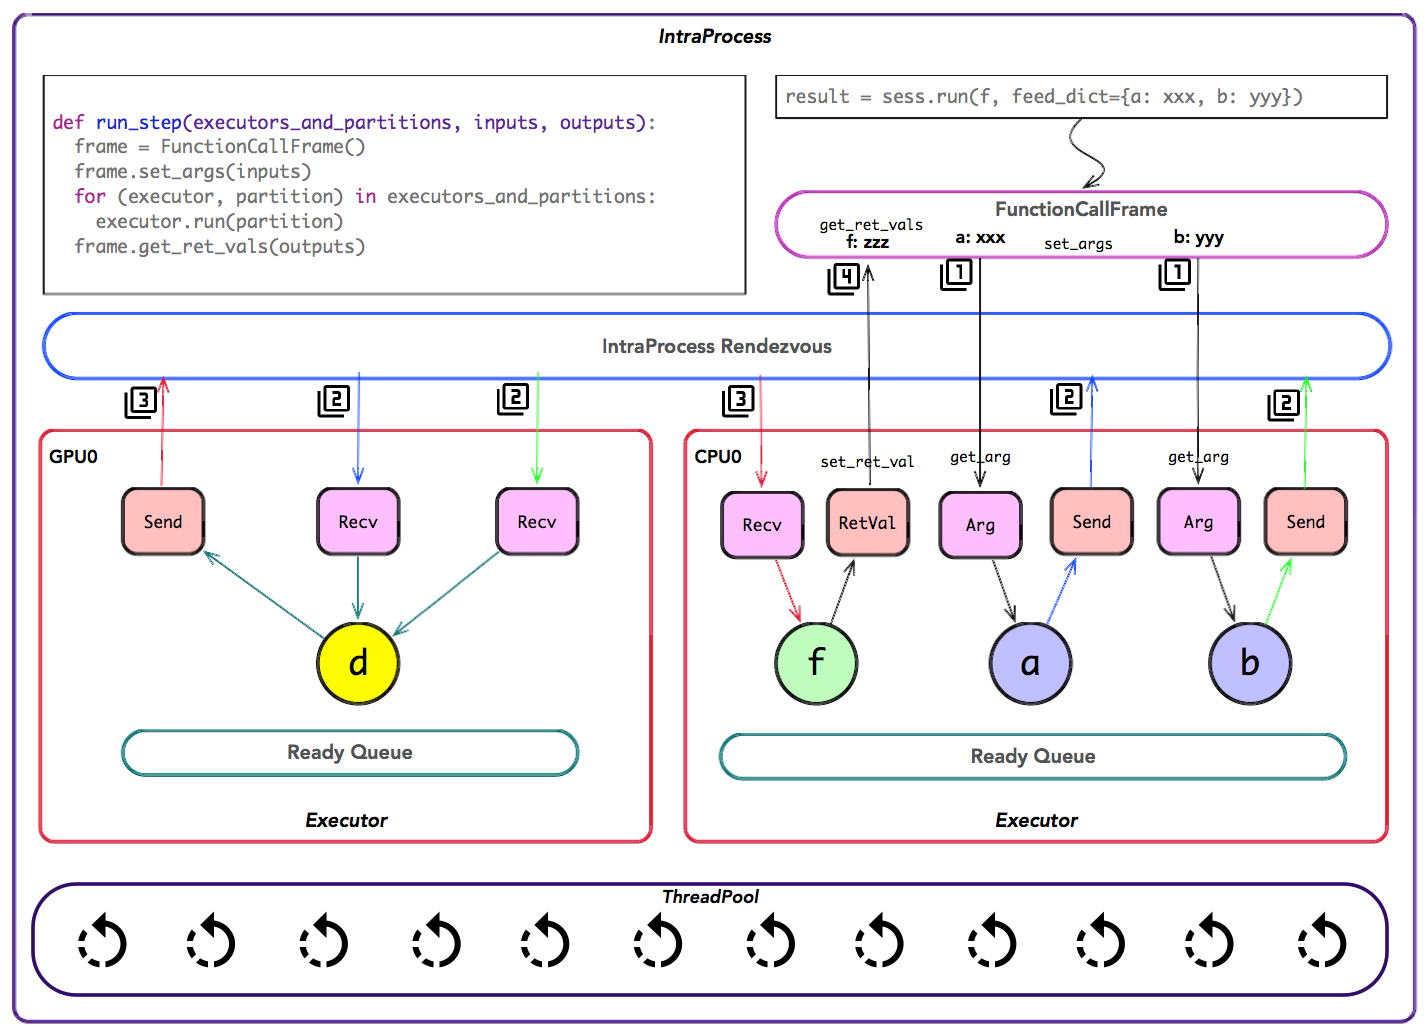
\includegraphics[width=1.0\textwidth]{figures/local-graph-execution.png}
\caption{执行图}
 \label{fig:local-graph-execution}
\end{figure}

因此,执行图计算需要解决如下\ascii{3}个核心问题:

\begin{enum}
  \eitem{输入/输出处理}
  \eitem{设备间数据交换} 
  \eitem{执行\code{PartitionGraph}}
\end{enum}

\subsection{输入}

在某个设备上,\code{PartitionGraph}的起始节点为\code{Arg}节点,结束节点为\code{RetVal}节点。整个过程可以看成函数调用过程,\code{Arg}用于传递函数参数,\code{RetVal}用于返回函数值。

更确切地说,\code{Arg}完成\code{PartitionGraph}的输入,\code{RetVal}完成
\code{PartitionGraph}的输出。对于\code{Arg}节点,其调用时序为:\code{set\_arg -> get\_arg}。其中,前者由\code{DirectSession}在启动\code{Executor}列表之前,通过调用\code{FunctionCallFrame.SetArgs(feeds)},传递输入参数列表的值;后者由\code{Arg}的\ascii{Kernel}实现调用。

\begin{leftbar}
\begin{c++}
Status DirectSession::Run(
  const RunOptions& run_options,
  const NamedTensorList& inputs,
  const std::vector<string>& output_names,
  const std::vector<string>& target_nodes,
  std::vector<Tensor>* outputs,
  RunMetadata* run_metadata) {

  // 1. prune graph
  // client\_graph = prune(full\_graph, inputs, outputs)
   
  // 2. split graph into partition by devices 
  // executors\_and\_partitions = split(client\_graph, devices)
  ExecutorsAndKeys* executors_and_keys = ... // ignore implements...
  
  // 3. lauch executor per partition
  // def run\_partitions(executors\_and\_partitions, inputs, outputs):
  // \ \ frame = FunctionCallFrame()
  // \ \ frame.set\_args(inputs)
  // \ \ for (executor, partition) in executors\_and\_partitions: 
  // \ \ \ \ exec.run(part)
  // \ \ frame.get\_ret\_vals(outputs)

  // 3.1 construct FunctionCallFrame
  FunctionCallFrame call_frame(
    executors_and_keys->input_types,
    executors_and_keys->output_types);
  
  // 3.2 frame.set\_args(inputs)
  // 3.2.1 construct feeds list
  gtl::InlinedVector<Tensor, 4> feed_args(inputs.size());
  for (const auto& it : inputs) {
    // (first, second) => (tensor\_name, tensor)
    feed_args[executors_and_keys->input_name_to_index[it.first]] = it.second;
  }

  // 3.2.2 frame.set\_args(feeds)
  call_frame.SetArgs(feed_args);
  
  // 3.3 concurent execution
  // for (executor, partition) in executors\_and\_partitions:
  // \ \ executor.run(partition) 

  // 3.4 fetch outputs.
}
\end{c++}
\end{leftbar}

而\code{frame.get\_arg}则有\code{Arg}来获取,并且\code{Arg}将其输出到\code{PartitionGraph}中的第一个计算节点。

\begin{leftbar}
\begin{c++}
struct ArgOp : OpKernel {
  explicit ArgOp(OpKernelConstruction* ctx) : OpKernel(ctx) {
    ctx->GetAttr("T", &dtype_);
    ctx->GetAttr("index", &index_);
  }

  void Compute(OpKernelContext* ctx) override {
    auto frame = ctx->call_frame();

    Tensor val;
    frame->GetArg(index_, &val);

    // put it into downsteram op's input.
    ctx->set_output(0, val); 
  }

 private:
  int index_;
  DataType dtype_;
};
\end{c++}
\end{leftbar}

\subsection{并发执行}

经过图分裂后,运行为每个\code{Partition}启动一个\code{Executor}。为了监听所有\code{Executor}是否全部完成,创建了一个\code{ExecutorBarrier}。并且在启动所有\code{Executor}之后,调用\code{executors\_done.Wait()}阻塞,等待所有\code{Executor}完成执行。

当完成一个\code{Executor}中完成,\code{ExecutorBarrier}的计算器减\ascii{1}(初始值为\code{num\_executors}),直至为\ascii{0},将调用其完成钩子,最终触发\code{executors\_done.Notify()}。

\begin{leftbar}
\begin{c++}
Status DirectSession::Run(
  const RunOptions& run_options,
  const NamedTensorList& inputs,
  const std::vector<string>& output_names,
  const std::vector<string>& target_nodes,
  std::vector<Tensor>* outputs,
  RunMetadata* run_metadata) {

  // 1. prune graph
  // client\_graph = prune(full\_graph, inputs, outputs)
   
  // 2. split graph into partition by devices 
  // executors\_and\_partitions = split(client\_graph, devices)
  ExecutorsAndKeys* executors_and_keys = ... // ignore implements...
  
  // 3. lauch executor per partition
  // def run\_partitions(executors\_and\_partitions, inputs, outputs):
  // \ \ frame = FunctionCallFrame()
  // \ \ frame.set\_args(inputs)
  // \ \ for (executor, partition) in executors\_and\_partitions: 
  // \ \ \ \ exec.run(part)
  // \ \ frame.get\_ret\_vals(outputs)

  // 3.1 construct FunctionCallFrame
  FunctionCallFrame call_frame(
    executors_and_keys->input_types,
    executors_and_keys->output_types);
  
  // 3.2 frame.set\_args(inputs)
  // 3.2.1 construct feeds list
  gtl::InlinedVector<Tensor, 4> feed_args(inputs.size());
  for (const auto& it : inputs) {
    // (first, second) => (tensor\_name, tensor)
    feed_args[executors_and_keys->input_name_to_index[it.first]] = it.second;
  }

  // 3.2.2 frame.set\_args(feeds)
  call_frame.SetArgs(feed_args);
  
  // 3.3 concurent execution
  // barrier = ExecutorBarrier(executors\_and\_partitions.size())
  // for (executor, partition) in executors\_and\_partitions:
  // \ \ executor.run(partition) 
  // barrier.wait()
  RunState run_state(&devices_);
  run_state.rendez = new IntraProcessRendezvous(device_mgr_.get());
  
  // 3.3.1 notify when finished.
  size_t num_executors = executors_and_keys->items.size();
  ExecutorBarrier* barrier = new ExecutorBarrier(
      num_executors, run_state.rendez, [&run_state](const Status& ret) {
        {
          mutex_lock l(run_state.mu_);
          run_state.status.Update(ret);
        }
        run_state.executors_done.Notify();
      });

  Executor::Args args;
  args.call_frame = &call_frame;
  args.rendezvous = run_state.rendez;
  args.runner = [this, pool](Executor::Args::Closure c) {
    SchedClosure(pool, std::move(c));
  };

  // 3.3.2 lauch all executors.
  for (const auto& item : executors_and_keys->items) {
    item.executor->RunAsync(args, barrier->Get());
  }

  // 3.3.3 wait until all executors finished.
  WaitForNotification(&run_state, 
      &step_cancellation_manager,
      GetTimeoutInMs(run_options));

  // 3.4 fetch outputs.
}
\end{c++}
\end{leftbar}

\subsection{输出}

同理,对于\code{RetVal}节点,其调用时序为:\code{set\_ret\_val -> get\_ret\_val}。前者由\code{RetVal}完成,后者由\code{DirectSession}完成。

\begin{leftbar}
\begin{c++}
struct RetvalOp : OpKernel {
  explicit RetvalOp(OpKernelConstruction* ctx) : OpKernel(ctx) {
    ctx->GetAttr("T", &dtype_);
    ctx->GetAttr("index", &index_);
  }

  void Compute(OpKernelContext* ctx) override {
    // get upstream op's output.
    const Tensor& val = ctx->input(0); 

    auto frame = ctx->call_frame();
    frame->SetRetval(index_, val);
  }

 private:
  int index_;
  DataType dtype_;
};
\end{c++}
\end{leftbar}

等所有\code{Executor}运行结束后,\code{DirectSession}便可以从\code{FunctionCallFrame}中取出所有输出值,并将其放置在\code{outputs},并返回\ascii{Client}。

\begin{leftbar}
\begin{c++}
Status DirectSession::Run(
  const RunOptions& run_options,
  const NamedTensorList& inputs,
  const std::vector<string>& output_names,
  const std::vector<string>& target_nodes,
  std::vector<Tensor>* outputs,
  RunMetadata* run_metadata) {
  
  // 1. prune graph
  // client\_graph = prune(full\_graph, inputs, outputs)
   
  // 2. split graph into partition by devices 
  // executors\_and\_partitions = split(client\_graph, devices)
  executors_and_keys = ... // ignore implements...
  
  // 3. lauch executor per partition
  // def run\_partitions(executors\_and\_partitions, inputs, outputs):
  // \ \ frame = FunctionCallFrame()
  // \ \ frame.set\_args(inputs)
  // \ \ for (executor, partition) in executors\_and\_partitions: 
  // \ \ \ \ exec.run(part)
  // \ \ frame.get\_ret\_vals(outputs)

  // 3.1 construct FunctionCallFrame
  FunctionCallFrame call_frame(
    executors_and_keys->input_types,
    executors_and_keys->output_types);
  
  // 3.2 frame.set\_args(inputs)
  // 3.2.1 construct feeds list
  gtl::InlinedVector<Tensor, 4> feed_args(inputs.size());
  for (const auto& it : inputs) {
    // (first, second) => (tensor\_name, tensor)
    feed_args[executors_and_keys->input_name_to_index[it.first]] = it.second;
  }

  // 3.2.2 frame.set\_args(feeds)
  call_frame.SetArgs(feed_args);
  
  // 3.3 concurent execution
  // barrier = ExecutorBarrier(executors\_and\_partitions.size())
  // for (executor, partition) in executors\_and\_partitions:
  // \ \ executor.run(partition) 
  // barrier.wait()
  RunState run_state(&devices_);
  run_state.rendez = new IntraProcessRendezvous(device_mgr_.get());
  
  // 3.3.1 notify when finished.
  size_t num_executors = executors_and_keys->items.size();
  ExecutorBarrier* barrier = new ExecutorBarrier(
      num_executors, run_state.rendez, [&run_state](const Status& ret) {
        {
          mutex_lock l(run_state.mu_);
          run_state.status.Update(ret);
        }
        run_state.executors_done.Notify();
      });

  Executor::Args args;
  args.call_frame = &call_frame;
  args.rendezvous = run_state.rendez;
  args.runner = [this, pool](Executor::Args::Closure c) {
    SchedClosure(pool, std::move(c));
  };

  // 3.3.2 lauch all executors.
  for (const auto& item : executors_and_keys->items) {
    item.executor->RunAsync(args, barrier->Get());
  }

  // 3.3.3 wait until all executors finished.
  WaitForNotification(&run_state, 
      &step_cancellation_manager,
      GetTimeoutInMs(run_options)); 

  // 3.4 fetch outputs. 
  // 3.4.1 frame.get\_get\_ret\_vals
  std::vector<Tensor> sorted_outputs;
  Status s = call_frame.ConsumeRetvals(&sorted_outputs);

  // 3.4.2 emplace to outputs, and return to client.
  outputs->reserve(sorted_outputs.size());
  for (int i = 0; i < output_names.size(); ++i) {
    const string& output_name = output_names[i];
    outputs->emplace_back(
      std::move(sorted_outputs[
        executors_and_keys->output_name_to_index[output_name]]));
  }
}
\end{c++}
\end{leftbar}

至此,整个\code{DirectSession.Run}解读完毕。但是,\code{Partition}中节点如何被调度执行的,\code{Partition}之间的\code{Send/Recv}是如何工作的呢?

因此,在最后一公里,还要探究三件事情。

\begin{enum}
  \eitem{\code{SendOp}与\code{RecvOp}的工作原理}
  \eitem{\code{IntraProcessRendezvous}的工作原理} 
  \eitem{\code{Executor}的调度算法}
\end{enum}

\section{设备间通信}

\code{SendOp/RecvOp}通过\code{Rendezvous}交换数据的;它实现了消息发送/接受,与具体消息传递相解耦。例如,在单进程内,\code{SendOp/RecvOp}基于\code{IntraProcessRendezvous}传递数据的;而在多进程环境中,\code{SendOp/RecvOp}则可以基于\code{GrpcRendezvous}传递数据。

首先,探究这两个\ascii{OP}的工作原理;然后,再探究本地模式下,\code{IntraProcessRendezvous}的工作原理。

\subsection{SendOp实现}

如\refig{local-send-recv-ops}所示,进程内的\code{Send/Recv}通过唯一的标识\code{ParsedKey}实现数据的交换。

\begin{figure}[H]
\centering
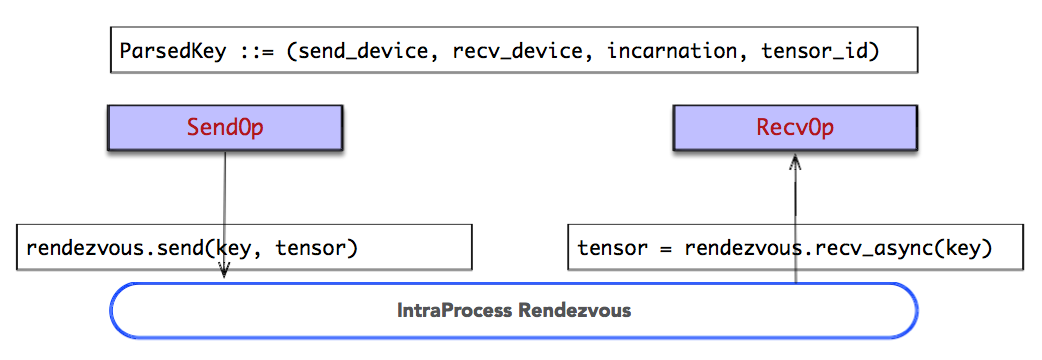
\includegraphics[width=0.8\textwidth]{figures/local-send-recv-ops.png}
\caption{进程内\code{SendOp}与\code{RecvOp}的数据交换}
 \label{fig:local-send-recv-ops}
\end{figure}

参考\code{SendOp}的\ascii{Kernel}实现,看起来非常复杂,但是它实际上就做了一件事情。首先,它构造设备间通信的关键字\code{ParsedKey},然后调用\code{Rendezvous.Send}操作,将上游\ascii{OP}输入到\code{SendOp}的\code{Tensor}发送到\code{Rendezvous}缓存之中,该操作是非阻塞的。

其中,\code{ParsedKey}包括:发送设备,接受设备,设备全局标识,及其待发送\code{Tensor}的标识(\code{src:output\_index})组成。

\begin{leftbar}
\begin{c++}
struct SendOp : OpKernel {
  explicit SendOp(OpKernelConstruction* ctx) : OpKernel(ctx) {
    string send_device;
    ctx->GetAttr("send_device", &send_device);

    string recv_device;
    ctx->GetAttr("recv_device", &recv_device);

    uint64 send_device_incarnation;
    ctx->GetAttr(
        "send_device_incarnation",
        reinterpret_cast<int64*>(&send_device_incarnation));

    string tensor_name;
    ctx->GetAttr("tensor_name", &tensor_name);

    key_prefix_ = GetRendezvousKeyPrefix(
        send_device, recv_device,
        send_device_incarnation, tensor_name);

    GetRendezvousKey(key_prefix_, {0, 0}, &parsed_key_.buf_);
    Rendezvous::ParseKey(parsed_key_.buf_, &parsed_key_);

    if (!ctx->GetAttr("_hostmem_sendrecv", &hostmem_sendrecv_).ok()) {
      hostmem_sendrecv_ = false;
    }
  }

  void Compute(OpKernelContext* ctx) override {
    Rendezvous::Args args;
    args.device_context = ctx->op_device_context();
    args.alloc_attrs = ctx->input_alloc_attr(0);
    
    // get it from upstream op's output, and as this op's input.
    ctx->rendezvous()->Send(
        CreateParsedkey(ctx), args, ctx->input(0),
        ctx->is_input_dead());
  }
 
 private:
  Rendezvous::ParsedKey CreateParsedkey(OpKernelContext* ctx) {
    FrameAndIter frame_iter = GetFrameAndIter(ctx, hostmem_sendrecv_);
    if (frame_iter == FrameAndIter(0, 0)) {
      return parsed_key_;
    } else {
      Rendezvous::ParsedKey in_loop_parsed;
      GetRendezvousKey(key_prefix_, frame_iter, &in_loop_parsed.buf_);
      Rendezvous::ParseKey(in_loop_parsed.buf_, &in_loop_parsed);
      return in_loop_parsed;
    }  
  }

 private:
  string key_prefix_;
  Rendezvous::ParsedKey parsed_key_;
  bool hostmem_sendrecv_;
};
\end{c++}
\end{leftbar}

\subsection{RecvOp实现}

同理地,可以猜测\code{Recv}的\ascii{Kernel}的实现了。它首先构造\code{Rendezvous}的\code{ParsedKey},然后调用\code{Rendezvous.RecvAsync}操作,从\code{Rendezvous}取出相应的\code{Tensor}。

这是一个异步操作,当\code{Rendezvous}中数据可获取,便开始执行回调函数\code{done\_cb},它将其得到的\code{Tensor}输出到下游\ascii{OP}。

\begin{leftbar}
\begin{c++}
struct RecvOp : AsyncOpKernel {
  explicit RecvOp(OpKernelConstruction* ctx) : AsyncOpKernel(ctx) {
    string send_device;
    ctx->GetAttr("send_device", &send_device);
  
    string recv_device;
    ctx->GetAttr("recv_device", &recv_device);

    uint64 send_device_incarnation;
    ctx->GetAttr(
        "send_device_incarnation",
        reinterpret_cast<int64*>(&send_device_incarnation));
  
    string tensor_name;
    ctx->GetAttr("tensor_name", &tensor_name);

    key_prefix_ = GetRendezvousKeyPrefix(
        send_device, recv_device,
        send_device_incarnation, tensor_name);
  
    GetRendezvousKey(key_prefix_, {0, 0}, &parsed_key_.buf_);
    Rendezvous::ParseKey(parsed_key_.buf_, &parsed_key_));
    if (!ctx->GetAttr("_hostmem_sendrecv", &hostmem_sendrecv_).ok()) {
      hostmem_sendrecv_ = false;
    }
  }

  void ComputeAsync(OpKernelContext* ctx, DoneCallback done) override {
    Rendezvous::Args args;
    args.device_context = ctx->op_device_context();
    args.alloc_attrs = ctx->output_alloc_attr(0);

    ctx->rendezvous()->RecvAsync(
      CreateParsedKey(ctx), args, CreateDoneCallback(ctx));
  }

 private:
  Rendezvous::ParsedKey CreateParsedKey(OpKernelContext* ctx) {
    FrameAndIter frame_iter = GetFrameAndIter(ctx, hostmem_sendrecv_);
    if (frame_iter == FrameAndIter(0, 0)) {
      return parsed_key_;
    } else {
      Rendezvous::ParsedKey in_loop_parsed;
      GetRendezvousKey(key_prefix_, frame_iter, &in_loop_parsed.buf_);
      Rendezvous::ParseKey(in_loop_parsed.buf_, &in_loop_parsed);
      return in_loop_parsed;
    }  
  }

  Rendezvous::DoneCallback CreateDoneCallback(OpKernelContext* ctx) {
    using namespace std::placeholders;
    return std::bind([ctx](DoneCallback done, const Status& s, 
        const Rendezvous::Args&, const Rendezvous::Args&, 
        const Tensor& val, bool is_dead) {
          ctx->SetStatus(s);
          if (s.ok()) {
            if (!is_dead) {
              // put it into downstream op's input.
              ctx->set_output(0, val);  
            }
            *ctx->is_output_dead() = is_dead;
          }
          done();
        },
        std::move(done), _1, _2, _3, _4, _5);  
  }

 private:
  string key_prefix_;
  Rendezvous::ParsedKey parsed_key_;
  bool hostmem_sendrecv_;
};
\end{c++}
\end{leftbar}
